% =====================================================================
%  The Scientific Discovery Engine -- a from-scratch guide
%  Build:  tectonic project_guide.tex      (run from the docs/ folder)
% =====================================================================
\documentclass[11pt,a4paper]{article}

\usepackage[T1]{fontenc}
\usepackage[utf8]{inputenc}
\usepackage{lmodern}
\usepackage[margin=2.2cm]{geometry}
\usepackage{amsmath,amssymb}
\usepackage{graphicx}
\usepackage{booktabs,longtable,array,tabularx}
\usepackage{enumitem}
\usepackage{xcolor}
\usepackage[most]{tcolorbox}
\usepackage{tikz}
\usetikzlibrary{arrows.meta,positioning,shapes.geometric,shapes.misc,fit,backgrounds,calc}
\usepackage{float}
\usepackage[section]{placeins}   % keep each phase's figures inside its section
\usepackage{caption}
\usepackage{microtype}
\usepackage[hidelinks]{hyperref}
\usepackage[strings,nohyphen]{underscore}  % function_names in plain text and TikZ nodes

\graphicspath{{../}}
\setlist{itemsep=2pt,topsep=4pt}
\setlength{\parskip}{4pt}
\setlength{\parindent}{0pt}

% Shared by project_guide.tex and submission_report.tex: macros, colours, flowchart styles, legend.
% Needs: xcolor, tikz (+ arrows.meta, positioning, shapes.geometric, shapes.misc, fit, backgrounds, calc),
% and the underscore package.

% ---------- code identifiers (underscores safe) ----------
\newcommand{\fn}[1]{\texttt{#1}}  % underscore pkg: _ prints literally and may break lines

% ---------- package colour palette (used in every flowchart) ----------
\definecolor{cData}{HTML}{6B7280}   % data/
\definecolor{cEqd}{HTML}{2563EB}    % equation_discovery/
\definecolor{cPinn}{HTML}{EA580C}   % pinn/
\definecolor{cVal}{HTML}{DC2626}    % validation/
\definecolor{cLlm}{HTML}{7C3AED}    % llm/
\definecolor{cHyp}{HTML}{15803D}    % hypotheses/
\definecolor{cRag}{HTML}{0D9488}    % rag/
\definecolor{cKg}{HTML}{92400E}     % knowledge_graph/
\definecolor{cEval}{HTML}{A16207}   % evaluation/
\definecolor{cExp}{HTML}{111827}    % experiments/

% ---------- flowchart styles ----------
\tikzset{
  >={Stealth[length=2.2mm]},
  fn/.style={draw=#1!75!black, fill=#1!10, rounded corners=2pt, line width=0.6pt,
             font=\ttfamily\scriptsize, align=center, inner sep=3pt, minimum height=6mm},
  fnw/.style={fn=#1, text width=47mm},
  stage/.style={draw=#1!75!black, fill=#1!8, rounded corners=3pt, line width=0.8pt,
                font=\small, align=left, inner sep=5pt, text width=0.80\textwidth},
  io/.style={draw=black!60, fill=black!4, font=\scriptsize\itshape, align=center,
             trapezium, trapezium left angle=75, trapezium right angle=105,
             inner sep=3pt, minimum height=6mm},
  dec/.style={draw=#1!75!black, fill=#1!10, diamond, aspect=2.4, font=\scriptsize,
              align=center, inner sep=1pt},
  note/.style={font=\scriptsize\itshape, text=black!65, align=left},
  flow/.style={->, line width=0.7pt, black!65},
  dflow/.style={->, line width=0.7pt, black!45, dashed},
  pkgbox/.style={draw=#1!60, fill=#1!4, rounded corners=4pt, line width=0.5pt, inner sep=6pt},
  pkglabel/.style={font=\ttfamily\scriptsize\bfseries, text=#1!80!black},
}

% legend used under every flowchart
\newcommand{\pkglegend}{%
  \par\smallskip\centering\scriptsize
  \tikz\node[fn=cData]{data};~\tikz\node[fn=cEqd]{equation\_discovery};~\tikz\node[fn=cPinn]{pinn};~%
  \tikz\node[fn=cVal]{validation};~\tikz\node[fn=cLlm]{llm};~\tikz\node[fn=cHyp]{hypotheses};\\[2pt]
  \tikz\node[fn=cRag]{rag};~\tikz\node[fn=cKg]{knowledge\_graph};~\tikz\node[fn=cEval]{evaluation};~%
  \tikz\node[fn=cExp]{experiments};\par}
   % macros, package colours, flowchart styles, legend

% ---------- teaching boxes ----------
\newtcolorbox{intuition}[1][]{colback=blue!3, colframe=blue!45!black, fonttitle=\bfseries\small,
  title={Intuition#1}, boxrule=0.6pt, arc=2pt, left=6pt, right=6pt, top=4pt, bottom=4pt}
\newtcolorbox{lesson}[1][]{colback=green!4, colframe=green!40!black, fonttitle=\bfseries\small,
  title={Key lesson#1}, boxrule=0.6pt, arc=2pt, left=6pt, right=6pt, top=4pt, bottom=4pt}
\newtcolorbox{incode}[1][]{colback=black!3, colframe=black!55, fonttitle=\bfseries\small,
  title={Where it lives in the code#1}, before upper=\raggedright, boxrule=0.6pt, arc=2pt, left=6pt, right=6pt, top=4pt, bottom=4pt}
\newtcolorbox{caution}[1][]{colback=red!3, colframe=red!50!black, fonttitle=\bfseries\small,
  title={Watch out#1}, boxrule=0.6pt, arc=2pt, left=6pt, right=6pt, top=4pt, bottom=4pt}

\title{\textbf{The Scientific Discovery Engine}\\[4pt]
\large A from-scratch guide to the project: the science, the code, every function,\\
and what actually happened in Phases 1--8 and the real Gemini run}
\author{Generated from the project source and its recorded results}
\date{October 2026}

\begin{document}
\maketitle
\thispagestyle{empty}

\begin{abstract}
\noindent This guide assumes you know a little Python and a little calculus, and nothing else about the
project. It first teaches the ideas the project is built from: partial differential equations, numerical
derivatives, sparse regression, physics-informed neural networks, large language models, retrieval and
knowledge graphs, and model selection. It then walks through the project phase by phase, explaining what was
built, which functions do the work, what the experiments found, and what each phase taught. Every phase has a
function-level flowchart, colour-coded by package. Appendix~\ref{app:functions} lists every function in the
codebase with a one-line description.
\end{abstract}

\tableofcontents
\clearpage

% =====================================================================
\section{The big picture in plain words}
% =====================================================================

\subsection{The question the project answers}

Imagine a long thin metal rod. At the start, some parts are hot and some are cold. You cannot watch the whole
rod continuously; instead, a few hundred cheap, noisy thermometer readings were taken at random places and
random times. Each reading is just three numbers:
\[
  (x,\; t,\; u) \;=\; (\text{position},\; \text{time},\; \text{measured temperature}).
\]
The question is: \textbf{what rule of nature produced these numbers?} Not ``draw a curve through the points'',
but ``find the \emph{law}'', the equation that says how $u$ changes in time at every point, so that you could
predict what happens at times and places nobody measured.

That is what this project calls \emph{scientific discovery}: given sparse, noisy observations of a field
$u(x,t)$, and \emph{not} the governing equation, recover the equation, estimate its unknown constants, reject
explanations that do not fit, and use the winner to predict outside the observed window.

\begin{intuition}[: a detective, not a curve-fitter]
A curve-fitter answers ``what numbers come next?''. A detective answers ``who did it, and how?''. This project
is built like a detective agency:
\begin{itemize}
  \item a \textbf{librarian} (RAG) fetches relevant textbook pages about how fields usually behave;
  \item an \textbf{archivist} (knowledge graph) keeps a structured card index of which mechanisms use which
        equations and parameters;
  \item a \textbf{brainstormer} (the LLM) suggests suspects: candidate equations;
  \item a \textbf{forensic lab} (physics-informed neural networks) tests each suspect against the evidence and
        estimates its unknown constants;
  \item a \textbf{judge} (model selection) picks the simplest suspect that fully explains the evidence;
  \item and a final \textbf{prediction test} checks the verdict on data that nobody used for any decision.
\end{itemize}
Crucially, the brainstormer is never allowed to decide the verdict. Only measured evidence decides.
\end{intuition}

\subsection{What the answer turned out to be}

The data was generated synthetically, so the true answer is known (but hidden from every decision):
\[
  \frac{\partial u}{\partial t} \;=\; D\,\frac{\partial^2 u}{\partial x^2}, \qquad D = 0.1 .
\]
This is the \emph{diffusion} (or heat) equation. In words: \emph{each point drifts towards the average of its
neighbours, at a speed set by $D$}. The project recovered this equation from 400 noisy points, estimated
$\hat D = 0.10002$ (0.02\% error), rejected the wrong candidates, and predicted the field beyond the observed
time window with an error of $2.5\times10^{-4}$. Phase~7 then repeated the whole pipeline on a different,
unseen system (advection--diffusion) and recovered both of its constants within 0.4\%.

\subsection{How the project was built: eight phases}

The project grew in phases, each adding one capability and each \emph{reporting its failures honestly}:

\begin{center}
\small
\begin{tabular}{@{}p{1.4cm}p{4.3cm}p{8.9cm}@{}}
\toprule
\textbf{Phase} & \textbf{Adds} & \textbf{One-line takeaway} \\ \midrule
1 & Synthetic data & Simulate diffusion, then sample 400 noisy points. A single-sine start turned out to be a trap. \\
2 & Equation discovery (SINDy) & Regression on numerical derivatives finds the law on clean data, fails on noisy data. \\
3 & PINNs & A neural network that must obey a candidate equation; it validates hypotheses and estimates $D$. \\
4 & Hypothesis generation (LLM) & An LLM proposes equations as structured JSON; a compiler turns any equation into a PINN. \\
5 & RAG + knowledge graph & Ground the LLM in retrieved textbook evidence, organised as a graph with provenance. \\
6 & Physics-constrained search & The full pipeline: pool $\to$ filters $\to$ PINN per candidate $\to$ selection $\to$ OOD. \\
7 & Evaluation & 12 benchmark datasets, 95 questions, 20 adversarial attacks, ablations, a second system. \\
8 & Final report & Audit of every claim: what was demonstrated and what was not. \\
+ & Real LLM (Gemini) & The mock LLM was replaced by Google Gemini for a real run (Section~\ref{sec:gemini}). \\
\bottomrule
\end{tabular}
\end{center}

\subsection{How to read this guide}

\begin{itemize}
  \item \textbf{Section~\ref{sec:background}} teaches every concept from zero. If a word in a later section is
        unfamiliar, it is explained there.
  \item \textbf{Section~\ref{sec:architecture}} shows the whole machine on one page, plus a map of how the code
        packages depend on each other.
  \item \textbf{Sections~\ref{sec:p1}--\ref{sec:p7}} walk through the phases. Each has a function-level flowchart.
        Boxes are coloured by the package the function lives in (legend under each chart). Solid arrows mean
        ``calls / passes data to''; dashed arrows mean ``feeds back'' or ``used later''.
  \item \textbf{Section~\ref{sec:gemini}} covers the real Gemini run and compares it with the mock LLM.
  \item \textbf{Appendix~\ref{app:functions}} is a complete function reference you can look things up in.
\end{itemize}

% =====================================================================
\section{Background crash course}\label{sec:background}
% =====================================================================

This section teaches, from zero, every idea the project uses. Each subsection ends with where the idea lives
in the code.

% ---------------------------------------------------------------------
\subsection{Fields and partial derivatives}

A \textbf{field} is a quantity that has a value at every place and time, written $u(x,t)$: the temperature
along a rod, the concentration of dye in a pipe, the density of a population along a coastline. Here $x$ is
one-dimensional (a line), so the whole field can be drawn as a heat-map with $x$ on one axis and $t$ on the
other.

A \textbf{partial derivative} measures how $u$ changes when you nudge \emph{one} variable and freeze the other.
The project writes them with subscripts, exactly as the code does:

\begin{center}
\begin{tabular}{@{}llp{9.2cm}@{}}
\toprule
\textbf{Code name} & \textbf{Maths} & \textbf{Meaning} \\ \midrule
\fn{u_t}   & $\partial u/\partial t$     & how fast the value at a fixed point is changing in time \\
\fn{u_x}   & $\partial u/\partial x$     & the slope of the profile at a fixed time (which way is ``uphill'') \\
\fn{u_xx}  & $\partial^2 u/\partial x^2$ & the curvature: positive in a valley, negative on a peak \\
\fn{u_xxx} & $\partial^3 u/\partial x^3$ & third derivative (in the library, never selected) \\
\bottomrule
\end{tabular}
\end{center}

\begin{intuition}[: curvature drives diffusion]
On a peak, the neighbours are lower than the point, so the curvature $u_{xx}$ is negative. In a valley the
neighbours are higher and $u_{xx}$ is positive. ``Move towards the average of your neighbours'' therefore
means ``change in time in proportion to the curvature'': $u_t = D\,u_{xx}$. Peaks sink, valleys fill, the
profile smooths out.
\end{intuition}

% ---------------------------------------------------------------------
\subsection{Partial differential equations (PDEs) and the four mechanism families}

A \textbf{PDE} is a rule connecting a field's partial derivatives. All the equations in this project are
\emph{evolution equations}: they say what $u_t$ is, given the current shape of $u$. The project works with four
mechanism families (and combinations of them):

\begin{center}
\small
\begin{tabular}{@{}p{3.0cm}p{4.2cm}p{7.6cm}@{}}
\toprule
\textbf{Family} & \textbf{Equation} & \textbf{What you would see} \\ \midrule
Diffusion & $u_t = D\,u_{xx}$ & Peaks flatten and spread; sharp features vanish fastest. $D>0$ is the diffusivity. \\
Advection & $u_t + c\,u_x = 0$ & The whole shape slides sideways at speed $c$ without changing shape. \\
Reaction (logistic) & $u_t = r\,u\,(1-u/K)$ & Each point grows (or decays) on its own towards a ceiling $K$; neighbours do not interact. \\
Advection--diffusion & $u_t + c\,u_x = D\,u_{xx}$ & The shape slides \emph{and} spreads: smoke drifting in wind. \\
Reaction--diffusion & $u_t = D\,u_{xx} + r\,u(1-u/K)$ & Spreading plus local growth: a population expanding into new territory. \\
\bottomrule
\end{tabular}
\end{center}

The letters $D, c, r, K$ are \textbf{parameters}: unknown constants that must be estimated from data. A
\textbf{hypothesis} in this project is an equation \emph{shape} (which terms appear) together with its unknown
parameters.

\begin{lesson}[: mechanism = which terms are present]
Identifying the mechanism means identifying \emph{which terms} the equation contains ($u_{xx}$? $u_x$? $u$ and
$u^2$?). Estimating parameters means finding their \emph{numbers}. The project scores these two separately,
because getting the numbers right does not prove you have the right terms (Section~\ref{sec:p7}).
\end{lesson}

% ---------------------------------------------------------------------
\subsection{Initial and boundary conditions, and well-posedness}

An evolution equation alone does not determine the future; you also need:
\begin{itemize}
  \item an \textbf{initial condition} (IC): the profile at $t=0$. Here
        $u(x,0) = \sin(\pi x) + 0.5\sin(3\pi x)$, a ``double hump'';
  \item \textbf{boundary conditions} (BC): what happens at the ends of the rod. Here $u(0,t)=u(1,t)=0$, the ends
        are held at zero (\emph{Dirichlet} conditions).
\end{itemize}
A problem is \textbf{well-posed} if a solution exists, is unique, and changes only a little when the data changes
a little. Two physical facts used later:
\begin{itemize}
  \item Diffusion with $D<0$ is the \emph{backward heat equation}: it un-mixes, and tiny wiggles explode. It is
        ill-posed, so the project enforces the physical bound $D>0$.
  \item Pure advection carries information in one direction only, so it can accept a boundary value only at the
        inflow end. Prescribing values at \emph{both} ends over-determines it; the project warns about this.
\end{itemize}

% ---------------------------------------------------------------------
\subsection{Simulating a PDE: finite differences}

Computers cannot handle a continuum, so the rod is cut into grid points $x_i$ spaced $\Delta x$ apart and time
into steps $\Delta t$. Derivatives become differences of neighbouring values:
\[
  u_{xx}(x_i) \approx \frac{u_{i+1} - 2u_i + u_{i-1}}{\Delta x^2}, \qquad
  u^{n+1}_i = u^n_i + \Delta t\, D\, \frac{u^n_{i+1} - 2u^n_i + u^n_{i-1}}{\Delta x^2}.
\]
The second formula is the \textbf{explicit (forward-time, centred-space) scheme} used to generate the data in
Phase~1. It is only stable if $D\,\Delta t/\Delta x^2 \le 1/2$, which is why the simulation uses 800 time
steps for 61 grid points. Later phases also need a general solver for \emph{any} candidate equation
(\fn{validation/forward_solver.py}); it offers simple Euler steps and the more accurate fourth-order
Runge--Kutta (RK4) method. Euler with centred differences is unconditionally unstable for advection, which is
why RK4 was added in Phase~7.

% ---------------------------------------------------------------------
\subsection{Numerical derivatives from data, and why noise is the enemy}

To \emph{discover} an equation from data you need the derivatives of the data. With scattered points you first
\textbf{reconstruct} a regular grid by interpolation, optionally \textbf{smooth} it, then take finite
differences. The trouble is that differencing amplifies noise. If each value has noise of size $\sigma$, the
second-difference formula divides by $\Delta x^2$, so its error is roughly
\[
  \text{error in } u_{xx} \;\sim\; \frac{\sigma}{\Delta x^2},
\]
which becomes enormous on a fine grid. A third derivative is worse still. Smoothing reduces the noise but
introduces bias. This single fact explains why Phase~2 works on clean data and fails on noisy data, and why the
project later turned to PINNs, which never take numerical differences of the data.

% ---------------------------------------------------------------------
\subsection{Sparse regression and SINDy}\label{sec:sindy}

\textbf{SINDy} (Sparse Identification of Nonlinear Dynamics) turns ``find the equation'' into a regression:
\begin{enumerate}
  \item Compute $u_t$ at many points: this is the target vector $y$.
  \item Build a \textbf{library} $\Theta$ whose columns are candidate terms evaluated at the same points. Here:
        $1,\ u,\ u_x,\ u_{xx},\ u_{xxx},\ u^2,\ u\,u_x,\ u\,u_{xx}$ (8 columns).
  \item Find coefficients $\xi$ with $y \approx \Theta\,\xi$, while forcing most entries of $\xi$ to be exactly
        zero, because real laws have few terms.
\end{enumerate}
The project's sparsifier is \textbf{STLSQ} (Sequentially Thresholded Least Squares): fit by ordinary least
squares, set every coefficient smaller than a threshold (0.05) to zero, refit using only the surviving
columns, and repeat until nothing changes. Columns are normalised first so the threshold means the same thing
for every term.

\begin{caution}[: identifiability and the eigenfunction trap]
Regression can only separate terms whose columns look different. For $\sin(\pi x)$, the second derivative is
$u_{xx} = -\pi^2 u$ \emph{exactly}, so the $u$ and $u_{xx}$ columns are perfectly proportional. No method can
tell $D\,u_{xx}$ apart from $-D\pi^2 u$. Phase~2 fell into exactly this trap with the original Phase~1 data and
``discovered'' $u_t = -0.987\,u$: a perfect fit, with the wrong physics. Using two sine modes with different
curvatures fixed it.
\end{caution}

% ---------------------------------------------------------------------
\subsection{Neural networks, automatic differentiation, and training}

A \textbf{multilayer perceptron} (MLP) is a function built from layers: each layer multiplies its input by a
weight matrix, adds a bias, and applies a squashing function (here $\tanh$). The project's network takes the two
numbers $(x,t)$ and outputs one number $u_\theta(x,t)$, where $\theta$ stands for all the weights. It has four
hidden layers of 64 units.

\textbf{Training} means adjusting $\theta$ to make a loss (an error score) small, using its gradient. The project
uses \textbf{Adam} (3000 steps, a robust first-order optimiser) and then \textbf{L-BFGS} (300 iterations, a
quasi-Newton method that converges much further once Adam is close).

\textbf{Automatic differentiation} (autograd, \fn{torch.autograd.grad}) gives \emph{exact} derivatives of the
network's output with respect to its inputs. So $\partial u_\theta/\partial t$ and
$\partial^2 u_\theta/\partial x^2$ come for free, with no finite differences and no noise amplification. This is
the key to PINNs.

% ---------------------------------------------------------------------
\subsection{Physics-informed neural networks (PINNs)}\label{sec:pinn}

A \textbf{PINN} is a neural network trained to do two things at once: pass close to the observations
\emph{and} obey a candidate equation everywhere. For a candidate written as a residual $\mathcal{R}=0$ (for
diffusion, $\mathcal{R} = u_t - D\,u_{xx}$) the loss is
\[
  \mathcal{L} \;=\;
  \underbrace{\tfrac1N\textstyle\sum_i \big(u_\theta(x_i,t_i) - u_i\big)^2}_{\text{data: fit observations}}
  + \underbrace{\tfrac1M\textstyle\sum_j \mathcal{R}(x_j,t_j)^2}_{\text{physics: obey the equation}}
  + \underbrace{\mathcal{L}_{\text{BC}}}_{\text{ends held at 0}}
  + \underbrace{\mathcal{L}_{\text{IC}}}_{\text{start profile}} .
\]
The physics term is evaluated at random \textbf{collocation points} $(x_j,t_j)$ that need no measurements.
All four weights are 1 in this project.
\begin{itemize}
  \item \textbf{Forward PINN:} the parameters are known (e.g.\ $D=0.1$ fixed). The PINN acts as a smart
        interpolator/denoiser that respects physics.
  \item \textbf{Inverse PINN:} the parameters are unknown. $D$ becomes a trainable number, optimised together
        with $\theta$. Whatever $D$ lets the network fit data \emph{and} physics best is the estimate.
\end{itemize}

\begin{intuition}[: why a PINN can reject a wrong equation]
If a candidate equation is wrong, no network can satisfy both the data and that equation at the same time;
one of the loss terms stays large. If it is right, all terms can be driven to near zero. So the final losses of a
trained inverse PINN are \emph{evidence} for or against the hypothesis, and the fitted parameters are estimates.
\end{intuition}

% ---------------------------------------------------------------------
\subsection{Large language models as hypothesis generators}

A \textbf{large language model} (LLM) such as Google Gemini predicts text. Given a description of what was
observed (``the amplitude decreased substantially, the peak did not move\ldots''), it can propose plausible
equations. The project treats the LLM strictly as a \emph{brainstormer}:
\begin{itemize}
  \item it must answer in \textbf{structured JSON} matching a schema (\fn{Hypothesis}: id, name, equation,
        parameters, required derivatives, mechanism, assumptions, rationale, confidence);
  \item its \fn{confidence} field is recorded but \emph{never} used as evidence;
  \item a deterministic validator checks syntax, variables, parameters and derivatives \emph{before} any
        expensive PINN training;
  \item the verdict comes only from measured PINN losses.
\end{itemize}
For testing without internet access, a \textbf{mock provider} returns a fixed, canned set of answers. All
Phase~4--7 numbers come from the mock; Section~\ref{sec:gemini} reports the real Gemini run.

% ---------------------------------------------------------------------
\subsection{Retrieval-augmented generation (RAG)}

\textbf{RAG} means: before asking the LLM, retrieve relevant documents and include them in the prompt, so its
proposals are grounded in evidence. The steps:
\begin{enumerate}
  \item \textbf{Corpus:} five short Markdown ``textbook'' documents, one per mechanism.
  \item \textbf{Chunking:} split each document at its section headers into chunks.
  \item \textbf{Embedding:} turn each chunk into a vector. The project uses a simple, deterministic
        \emph{bag-of-words hashing} embedding: each word is hashed into one of 256 slots, slot counts form the
        vector, and the vector is normalised to length 1.
  \item \textbf{Search:} embed the query (the observation description) the same way and return the chunks with
        the highest \emph{cosine similarity} (the dot product of unit vectors).
\end{enumerate}
\textbf{Answer leakage} is the danger that retrieved text gives away the answer. The corpus states only generic
textbook laws (``Fick's second law, $u_t = D\,u_{xx}$'') and never this dataset's value $D=0.1$; an automated
check verifies this.

% ---------------------------------------------------------------------
\subsection{Knowledge graphs}

A \textbf{knowledge graph} stores facts as typed nodes and typed edges: \emph{Mechanism} ``diffusion''
\textsc{governs} \emph{Equation} ``$u_t=D\,u_{xx}$'', which \textsc{has\_parameter} \emph{Parameter} ``$D$'',
\textsc{supported\_by} \emph{Document} ``diffusion.md''. Every edge records its \textbf{provenance} (which
document and chunk it came from). Where RAG answers ``what text is relevant?'', the graph answers structured
questions such as ``which parameters appear in the documented equations for diffusion?'' (answer: $D$). In this
project the graph has 22 entities and 40 relationships, all sourced, and it supplies \emph{equation templates}
that join the LLM's proposals in the candidate pool.

% ---------------------------------------------------------------------
\subsection{Choosing between hypotheses: splits, parsimony, BIC}\label{sec:selection}

\textbf{Data splits.} To judge a model honestly you must test it on data it never saw:
\begin{itemize}
  \item \textbf{train:} used to fit (observations with $t \le 0.8$, minus a holdout);
  \item \textbf{validation (held-out):} a random 20\% of the $t\le0.8$ points, used for the accept/reject
        \emph{gate} and for selection;
  \item \textbf{OOD (out-of-distribution):} all points with $t>0.8$, never used to train or select. It
        measures genuine extrapolation into the future.
\end{itemize}

\textbf{Nested models.} Reaction--diffusion with $r=0$ \emph{is} diffusion; advection--diffusion with $c=0$
\emph{is} diffusion. A more general model can always fit at least as well, so ``best fit'' alone favours
needless complexity. This is the \emph{nested-model problem}.

\textbf{Parsimony (Occam's razor).} Among models that fit equally well, prefer the simplest. The project makes
this precise:
\begin{enumerate}
  \item \emph{Gate:} reject a candidate unless its held-out error, physics residual, BC/IC losses and physical
        bounds are all within fixed thresholds.
  \item \emph{Equivalence:} keep the gate survivors whose held-out RMSE is within 5\% of the best.
  \item \emph{Complexity:} choose the lowest score
        $=\#\text{terms} + \#\text{free parameters} + \text{max derivative order} + 2\cdot\#\text{nonlinear terms}
        + 0.1\cdot\#\text{operations}$.
  \item \emph{BIC} as a tie-breaker and cross-check: $\text{BIC} = n\ln(\text{MSE}) + k\ln n$, which rewards
        fit and charges $\ln n$ per parameter.
\end{enumerate}

\textbf{Term necessity.} For each parameter, measure what share of $u_t$ (RMS) its terms contribute on the
trained PINN. Below 5\% the parameter is \emph{inactive}: the data does not need that term. Phase~7 promoted
this into the selection rule (Section~\ref{sec:p7}).

\textbf{The oracle rule.} Because the data is synthetic, the clean truth is known. It may be used \emph{only}
to report error \emph{after} every decision has been made (the function \fn{oracle_evaluation}), never to make a
decision. Phase~7 audits the code automatically for violations of this rule.

\begin{incode}
Derivatives: \fn{equation_discovery/derivatives.py} (finite differences) and \fn{pinn/derivatives.py}
(autograd). SINDy: \fn{equation_discovery/sindy.py}. PINN: \fn{pinn/}. LLM: \fn{llm/}. RAG: \fn{rag/}.
Graph: \fn{knowledge_graph/}. Selection: \fn{validation/model_selection.py}, \fn{hypotheses/complexity.py}.
Splits and the gate: \fn{hypotheses/search.py}.
\end{incode}

% =====================================================================
\section{The whole machine on one page}\label{sec:architecture}
% =====================================================================

Figure~\ref{fig:pipeline} is the complete discovery pipeline as finally assembled in Phase~6. Read it top to
bottom: each stage hands its output to the next. The right-hand column says which package does the work and
which question the stage answers.

\begin{figure}[!htb]
\centering
% flowchart 'pipeline' -- used by docs/Report.tex
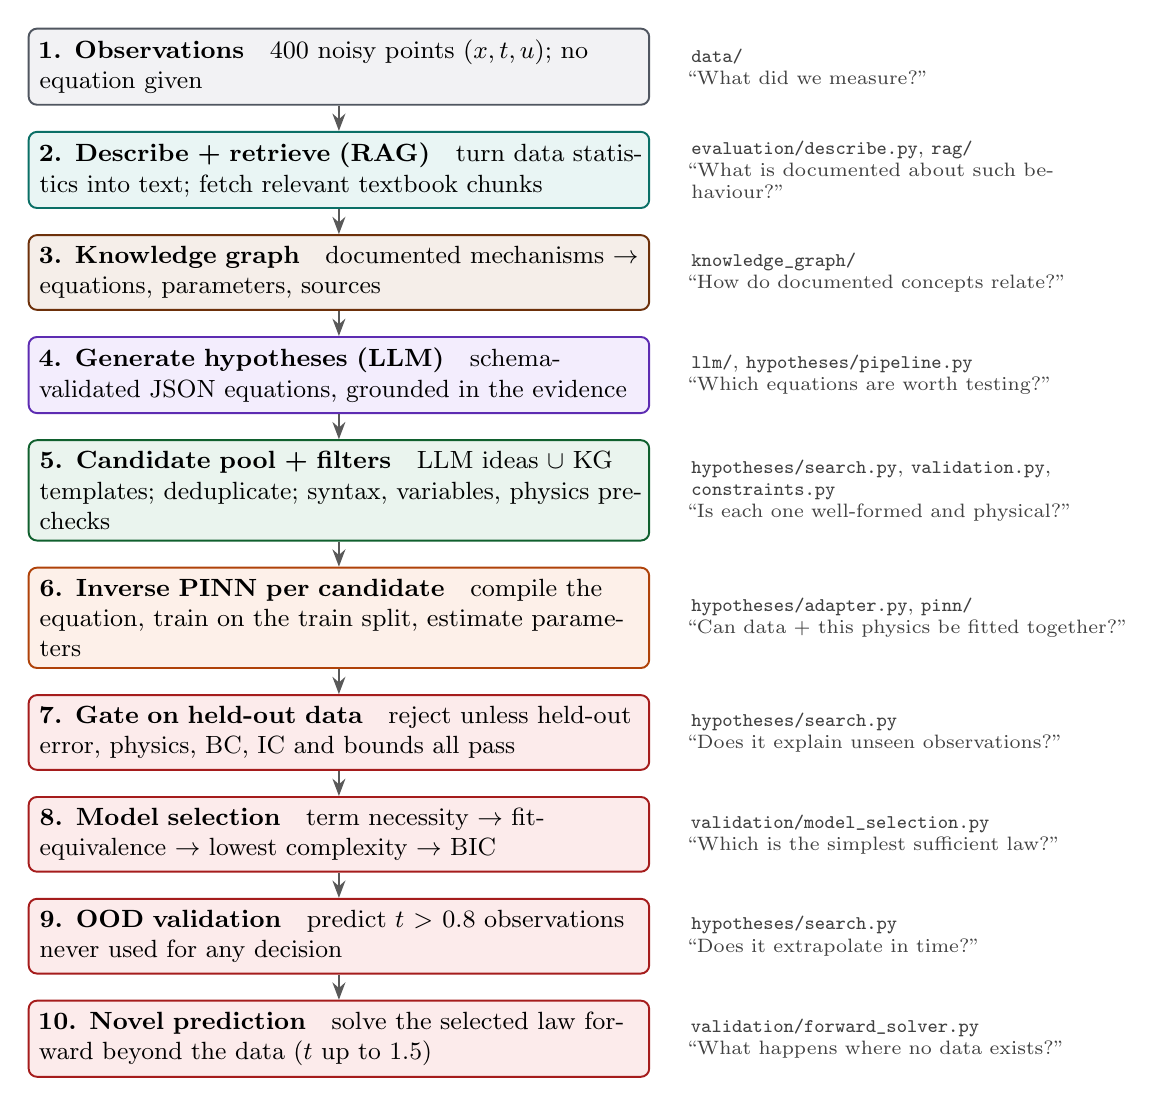
\begin{tikzpicture}[node distance=3.2mm]
  \tikzset{st/.style={draw=#1!75!black, fill=#1!9, rounded corners=3pt, line width=0.7pt,
                      font=\small, align=left, inner sep=4pt, text width=7.6cm},
           side/.style={font=\scriptsize, align=left, text width=5.6cm, text=black!75}}
  \node[st=cData] (s1) {\textbf{1. Observations}\quad 400 noisy points $(x,t,u)$; no equation given};
  \node[st=cRag, below=of s1] (s2) {\textbf{2. Describe + retrieve (RAG)}\quad turn data statistics into
        text; fetch relevant textbook chunks};
  \node[st=cKg, below=of s2] (s3) {\textbf{3. Knowledge graph}\quad documented mechanisms $\to$ equations,
        parameters, sources};
  \node[st=cLlm, below=of s3] (s4) {\textbf{4. Generate hypotheses (LLM)}\quad schema-validated JSON
        equations, grounded in the evidence};
  \node[st=cHyp, below=of s4] (s5) {\textbf{5. Candidate pool + filters}\quad LLM ideas $\cup$ KG templates;
        deduplicate; syntax, variables, physics pre-checks};
  \node[st=cPinn, below=of s5] (s6) {\textbf{6. Inverse PINN per candidate}\quad compile the equation, train
        on the train split, estimate parameters};
  \node[st=cVal, below=of s6] (s7) {\textbf{7. Gate on held-out data}\quad reject unless held-out error,
        physics, BC, IC and bounds all pass};
  \node[st=cVal, below=of s7] (s8) {\textbf{8. Model selection}\quad term necessity $\to$ fit-equivalence
        $\to$ lowest complexity $\to$ BIC};
  \node[st=cVal, below=of s8] (s9) {\textbf{9. OOD validation}\quad predict $t>0.8$ observations never used
        for any decision};
  \node[st=cVal, below=of s9] (s10) {\textbf{10. Novel prediction}\quad solve the selected law forward beyond
        the data ($t$ up to 1.5)};
  \foreach \a/\b in {s1/s2,s2/s3,s3/s4,s4/s5,s5/s6,s6/s7,s7/s8,s8/s9,s9/s10}
     \draw[flow] (\a) -- (\b);
  \node[side, right=4mm of s1]  {\fn{data/}\\ ``What did we measure?''};
  \node[side, right=4mm of s2]  {\fn{evaluation/describe.py}, \fn{rag/}\\ ``What is documented about such behaviour?''};
  \node[side, right=4mm of s3]  {\fn{knowledge_graph/}\\ ``How do documented concepts relate?''};
  \node[side, right=4mm of s4]  {\fn{llm/}, \fn{hypotheses/pipeline.py}\\ ``Which equations are worth testing?''};
  \node[side, right=4mm of s5]  {\fn{hypotheses/search.py}, \fn{validation.py}, \fn{constraints.py}\\ ``Is each one well-formed and physical?''};
  \node[side, right=4mm of s6]  {\fn{hypotheses/adapter.py}, \fn{pinn/}\\ ``Can data + this physics be fitted together?''};
  \node[side, right=4mm of s7]  {\fn{hypotheses/search.py}\\ ``Does it explain unseen observations?''};
  \node[side, right=4mm of s8]  {\fn{validation/model_selection.py}\\ ``Which is the simplest sufficient law?''};
  \node[side, right=4mm of s9]  {\fn{hypotheses/search.py}\\ ``Does it extrapolate in time?''};
  \node[side, right=4mm of s10] {\fn{validation/forward_solver.py}\\ ``What happens where no data exists?''};
\end{tikzpicture}

\caption{The end-to-end discovery pipeline (Phase~6 form). Colours follow the package legend used in every
flowchart.}
\label{fig:pipeline}
\end{figure}

\begin{lesson}[: who is allowed to decide]
\begin{itemize}
  \item RAG \emph{retrieves}, the graph \emph{organises}, the LLM \emph{proposes}. None of them can mark an
        equation as correct; there is literally no field for that in the schema.
  \item Ranking (\fn{hypotheses/ranking.py}) only sets the \emph{order} in which candidates are examined.
  \item Only measured numbers decide: the gate (\fn{validate_candidate}) and \fn{select_model}, both using
        held-out \emph{noisy} observations, never the hidden truth.
  \item Status strings are deliberately modest: ``supported by the available observations and physics
        constraints'' or ``rejected under the tested conditions''. Never ``proven''.
\end{itemize}
\end{lesson}

\subsection{How the code packages depend on each other}

Figure~\ref{fig:packages} was computed from the actual \fn{import} statements in the code. An arrow
$A\to B$ means ``package $A$ imports from package $B$''. Double-headed arrows are mutual imports.

\begin{figure}[!htb]
\centering
% flowchart 'packages' -- used by docs/Report.tex
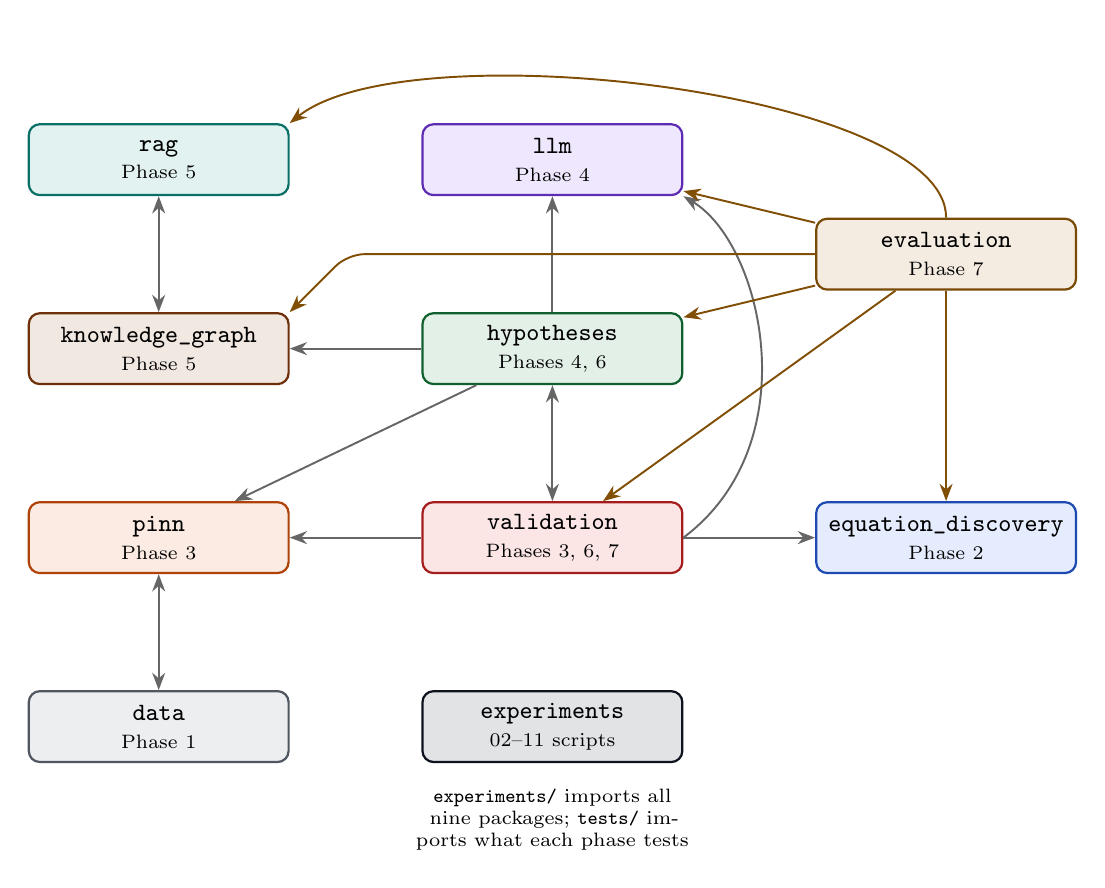
\begin{tikzpicture}[
   pk/.style={draw=#1!75!black, fill=#1!12, rounded corners=4pt, line width=0.8pt,
              font=\ttfamily\small\bfseries, minimum width=3.3cm, minimum height=9mm, align=center},
   dep/.style={->, line width=0.7pt, black!60},
   mdep/.style={<->, line width=0.7pt, black!60}]
  \node[pk=cRag]  (rag) at (0,0)     {rag\\[-1pt]{\normalfont\scriptsize Phase 5}};
  \node[pk=cKg]   (kg)  at (0,-2.4)  {knowledge\_graph\\[-1pt]{\normalfont\scriptsize Phase 5}};
  \node[pk=cLlm]  (llm) at (5,0)     {llm\\[-1pt]{\normalfont\scriptsize Phase 4}};
  \node[pk=cHyp]  (hyp) at (5,-2.4)  {hypotheses\\[-1pt]{\normalfont\scriptsize Phases 4, 6}};
  \node[pk=cVal]  (val) at (5,-4.8)  {validation\\[-1pt]{\normalfont\scriptsize Phases 3, 6, 7}};
  \node[pk=cPinn] (pinn) at (0,-4.8) {pinn\\[-1pt]{\normalfont\scriptsize Phase 3}};
  \node[pk=cData] (data) at (0,-7.2) {data\\[-1pt]{\normalfont\scriptsize Phase 1}};
  \node[pk=cEqd]  (eqd) at (10,-4.8) {equation\_discovery\\[-1pt]{\normalfont\scriptsize Phase 2}};
  \node[pk=cEval] (ev)  at (10,-1.2) {evaluation\\[-1pt]{\normalfont\scriptsize Phase 7}};
  \node[pk=cExp]  (exp) at (5,-7.2)  {experiments\\[-1pt]{\normalfont\scriptsize 02--11 scripts}};

  \draw[mdep] (rag) -- (kg);
  \draw[mdep] (pinn) -- (data);
  \draw[mdep] (hyp) -- (val);
  \draw[dep] (hyp) -- (kg);
  \draw[dep] (hyp) -- (llm);
  \draw[dep] (hyp) -- (pinn);
  \draw[dep] (val) -- (pinn);
  \draw[dep] (val) -- (eqd);
  \draw[dep] (val.east) .. controls +(1.6,1.2) and +(1.0,-0.6) .. (llm.south east);
  \draw[dep, cEval!80!black] (ev) -- (llm);
  \draw[dep, cEval!80!black] (ev) -- (hyp);
  \draw[dep, cEval!80!black] (ev) -- (eqd);
  \draw[dep, cEval!80!black] (ev) -- (val);
  \draw[dep, cEval!80!black] (ev.north) .. controls +(0,1.6) and +(1.5,1.2) .. (rag.north east);
  \draw[dep, cEval!80!black, rounded corners=6pt] (ev.west) -- (2.4,-1.2) -- (kg.north east);
  \node[font=\scriptsize, align=center, text width=4.4cm, below=2mm of exp]
       {\fn{experiments/} imports all nine packages; \fn{tests/} imports what each phase tests};
\end{tikzpicture}

\caption{Package dependency map, derived from the real imports. The phase that introduced each package is shown
under its name.}
\label{fig:packages}
\end{figure}

\begin{intuition}[: reading the map]
\fn{hypotheses} sits in the middle because it glues the brainstormer (\fn{llm}) to the lab (\fn{pinn}) and the
judge (\fn{validation}). \fn{evaluation} (Phase~7) reaches into almost everything because it re-runs the whole
pipeline on benchmark datasets. \fn{data} and \fn{pinn} import each other only because the problem description
and the PINN share the same data-loading helper (\fn{load_observational_data}).
\end{intuition}

% =====================================================================
\section{Phase 1: making the data}\label{sec:p1}
% =====================================================================

\textbf{Goal.} Produce realistic observations of a known law, so that every later phase can be graded against
a truth it is not allowed to see.

\textbf{What happens.} \fn{data/generate_diffusion.py} simulates $u_t = 0.1\,u_{xx}$ on $x\in[0,1]$,
$t\in[0,1]$ with the explicit finite-difference scheme (61 grid points $\times$ 800 time steps), starting
from the double hump $\sin(\pi x) + 0.5\sin(3\pi x)$ with both ends held at zero. From the full field it
saves three files:

\begin{center}
\small
\begin{tabular}{@{}lp{11.5cm}@{}}
\toprule
\fn{full.npz} & the entire clean field (800$\times$61). For grading and plots only. \\
\fn{sparse.npz} & a noise-free random 10\% of grid points (4880 points). For ablations of sparsity alone. \\
\fn{noisy.npz} & \textbf{400 random points with Gaussian noise} (std = 5\% of the field's std, $\approx0.0116$).
                 \textbf{The only file the discovery system may see}, and it uses only its $x,t,u$ columns. \\
\bottomrule
\end{tabular}
\end{center}

\begin{figure}[!htb]
\centering
% flowchart 'p1' -- shared by project_guide.tex and submission_report.tex
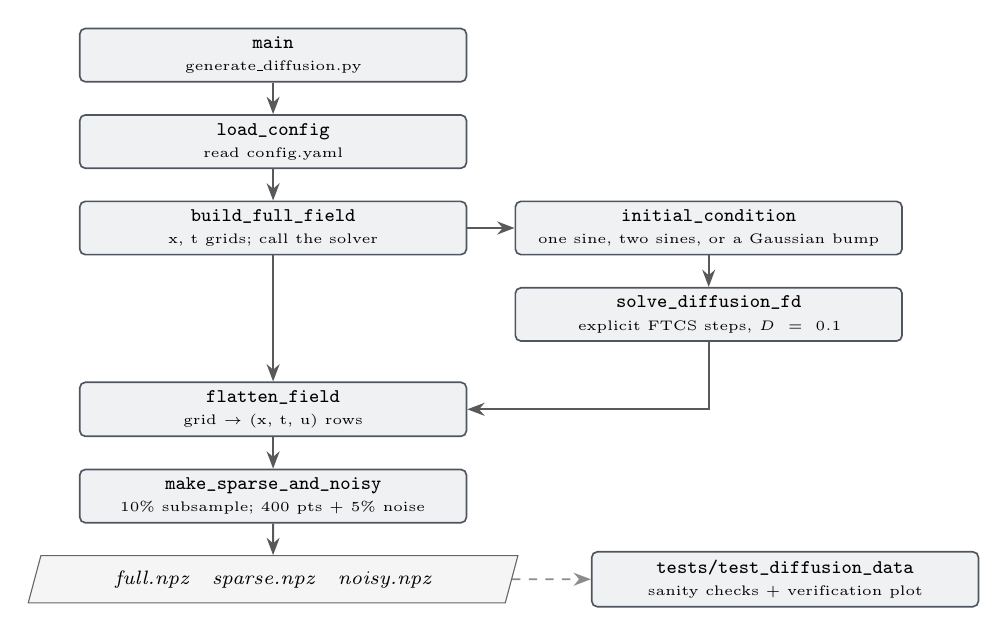
\begin{tikzpicture}[node distance=4mm and 6mm]
  \node[fnw=cData] (main) {main\\{\normalfont\tiny generate\_diffusion.py}};
  \node[fnw=cData, below=of main] (cfg) {load_config\\{\normalfont\tiny read config.yaml}};
  \node[fnw=cData, below=of cfg] (full) {build_full_field\\{\normalfont\tiny x, t grids; call the solver}};
  \node[fnw=cData, right=of full] (ic) {initial_condition\\{\normalfont\tiny one sine, two sines, or a Gaussian bump}};
  \node[fnw=cData, below=of ic] (fd) {solve_diffusion_fd\\{\normalfont\tiny explicit FTCS steps, $D=0.1$}};
  \node[fnw=cData, below=of full, yshift=-12mm] (flat) {flatten_field\\{\normalfont\tiny grid $\to$ (x, t, u) rows}};
  \node[fnw=cData, below=of flat] (samp) {make_sparse_and_noisy\\{\normalfont\tiny 10\% subsample; 400 pts + 5\% noise}};
  \node[io, below=of samp] (files) {full.npz\quad sparse.npz\quad noisy.npz};
  \node[fnw=cData, right=of files, xshift=4mm] (test) {tests/test_diffusion_data\\{\normalfont\tiny sanity checks + verification plot}};
  \draw[flow] (main) -- (cfg); \draw[flow] (cfg) -- (full);
  \draw[flow] (full) -- (ic); \draw[flow] (ic) -- (fd); \draw[flow] (fd) |- (flat);
  \draw[flow] (full) -- (flat); \draw[flow] (flat) -- (samp); \draw[flow] (samp) -- (files);
  \draw[dflow] (files) -- (test);
\end{tikzpicture}

\pkglegend
\caption{Phase~1 function flow: configuration $\to$ simulation $\to$ sampling $\to$ files $\to$ checks.}
\label{fig:p1}
\end{figure}

\begin{figure}[!htb]
\centering
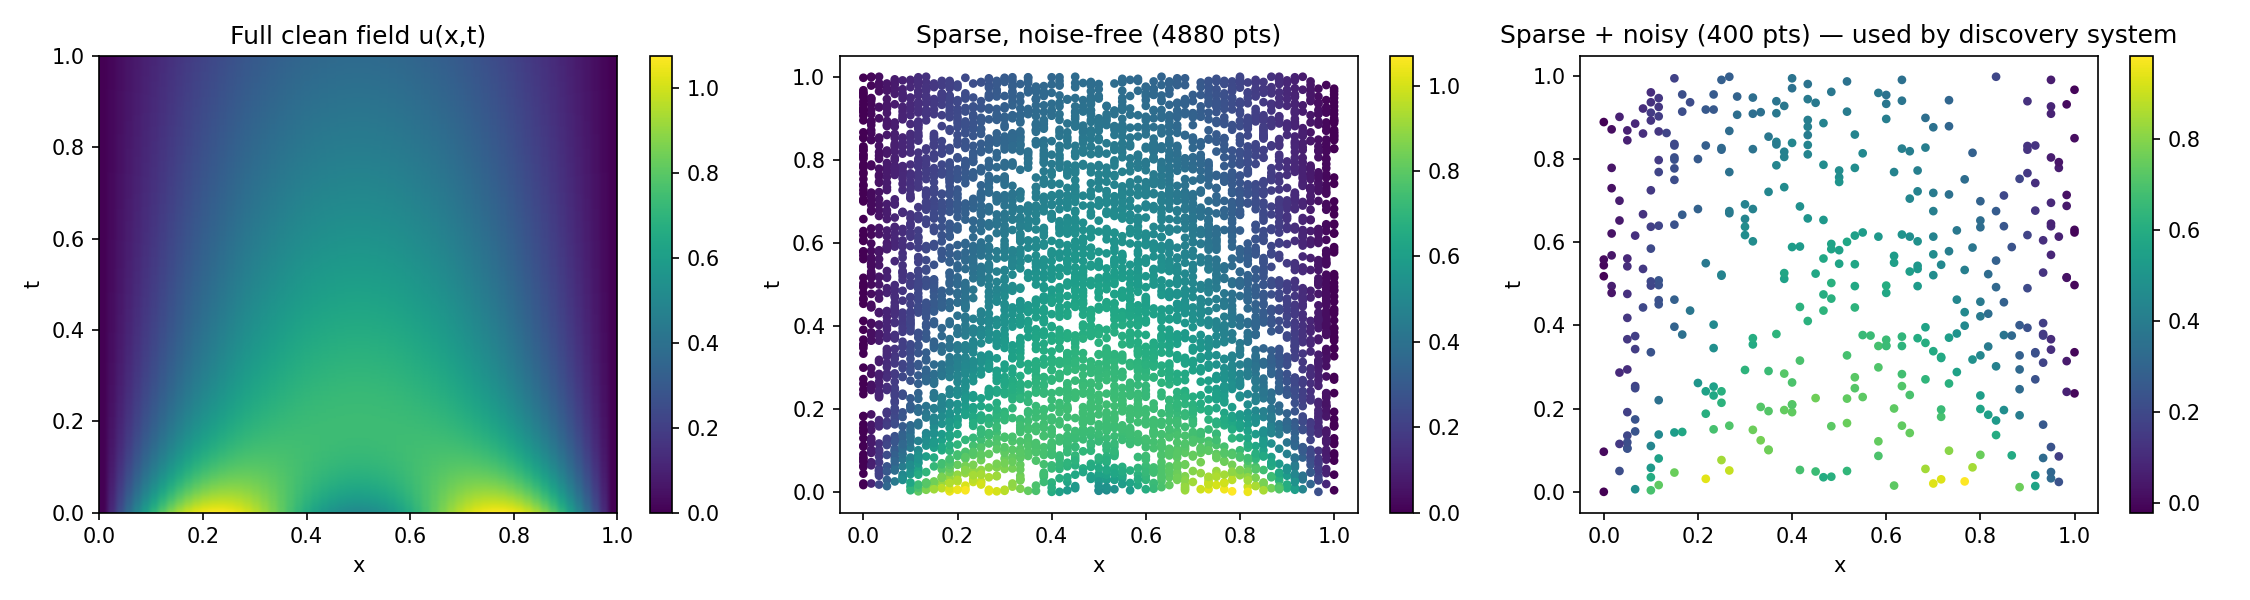
\includegraphics[width=0.95\textwidth]{data/generated/verification_plot.png}
\caption{Phase~1 verification plot (from the project's results): the clean field (left), the sparse sample, and
the 400 noisy points the system is allowed to see. The double hump decays and merges into one broad hump,
because the faster-wiggling mode $\sin(3\pi x)$ decays 9 times faster than $\sin(\pi x)$.}
\end{figure}

\begin{lesson}[: the eigenfunction trap]
The first version started from a single $\sin(\pi x)$. That turned out to be undiscoverable: for this profile
$u_{xx}=-\pi^2u$ exactly, so ``$D\,u_{xx}$'' and ``$-D\pi^2u$'' are the same signal and no method can separate
them. The two-mode start mixes two different curvatures and breaks the tie. The single-mode option is kept in
the code as a documented cautionary example, and Phase~7's adversarial suite re-tests it (case A13).
\end{lesson}

% =====================================================================
\section{Phase 2: equation discovery by sparse regression}\label{sec:p2}
% =====================================================================

\textbf{Goal.} Recover $u_t \approx D\,u_{xx}$ from data alone using SINDy (Section~\ref{sec:sindy}), and
report honestly where it works and where it does not.

\textbf{How it works.} For clean data (already a grid), take finite differences directly. For scattered data,
first reconstruct a grid by linear interpolation (41$\times$150 nodes for 4880 sparse points, but only
13$\times$25 for 400 noisy points), optionally smooth it with a Gaussian filter, then difference. Build the
8-column library and run STLSQ with threshold 0.05.

\begin{figure}[!htb]
\centering
% flowchart 'p2' -- used by docs/Report.tex
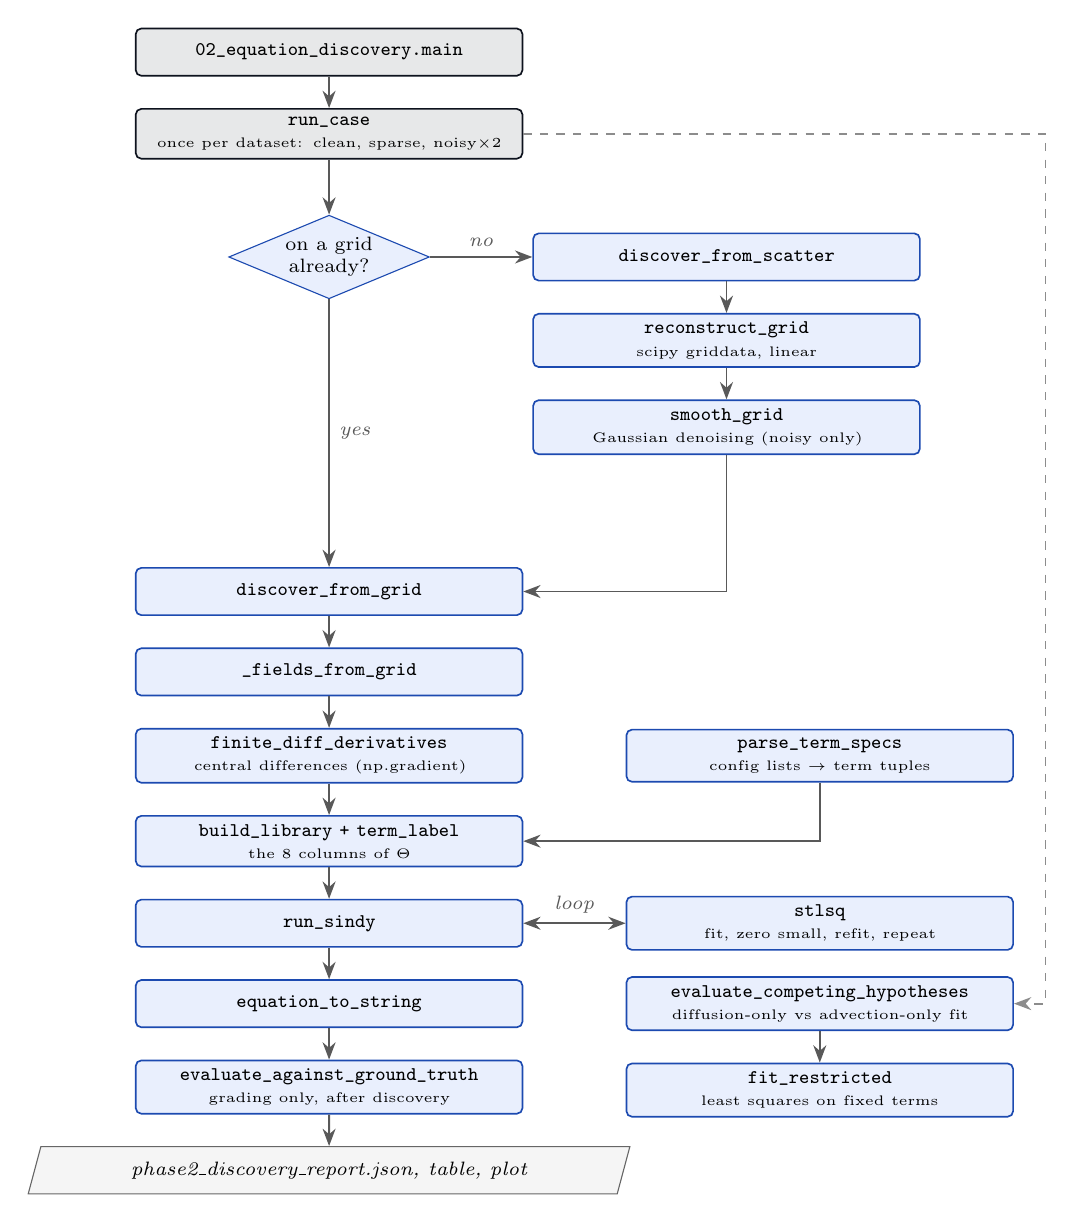
\begin{tikzpicture}[node distance=4mm and 7mm]
  \node[fnw=cExp] (main) {02_equation_discovery.main};
  \node[fnw=cExp, below=of main] (case) {run_case\\{\normalfont\tiny once per dataset: clean, sparse, noisy$\times$2}};
  \node[dec=cEqd, below=7mm of case] (q) {on a grid\\already?};
  \node[fnw=cEqd, right=of q, xshift=6mm] (scat) {discover_from_scatter};
  \node[fnw=cEqd, below=of scat] (rec) {reconstruct_grid\\{\normalfont\tiny scipy griddata, linear}};
  \node[fnw=cEqd, below=of rec] (sm) {smooth_grid\\{\normalfont\tiny Gaussian denoising (noisy only)}};
  \node[fnw=cEqd, below=34mm of q] (grid) {discover_from_grid};
  \node[fnw=cEqd, below=of grid] (fields) {_fields_from_grid};
  \node[fnw=cEqd, below=of fields] (fdd) {finite_diff_derivatives\\{\normalfont\tiny central differences (np.gradient)}};
  \node[fnw=cEqd, right=of fdd, xshift=6mm] (specs) {parse_term_specs\\{\normalfont\tiny config lists $\to$ term tuples}};
  \node[fnw=cEqd, below=of fdd] (lib) {build_library + term_label\\{\normalfont\tiny the 8 columns of $\Theta$}};
  \node[fnw=cEqd, below=of lib] (sindy) {run_sindy};
  \node[fnw=cEqd, right=of sindy, xshift=6mm] (stlsq) {stlsq\\{\normalfont\tiny fit, zero small, refit, repeat}};
  \node[fnw=cEqd, below=of sindy] (str) {equation_to_string};
  \node[fnw=cEqd, below=of str] (gt) {evaluate_against_ground_truth\\{\normalfont\tiny grading only, after discovery}};
  \node[fnw=cEqd, right=of str, xshift=6mm] (comp) {evaluate_competing_hypotheses\\{\normalfont\tiny diffusion-only vs advection-only fit}};
  \node[fnw=cEqd, below=of comp] (restr) {fit_restricted\\{\normalfont\tiny least squares on fixed terms}};
  \node[io, below=of gt] (out) {phase2\_discovery\_report.json, table, plot};
  \draw[flow] (main) -- (case); \draw[flow] (case) -- (q);
  \draw[flow] (q) -- node[note, above]{no} (scat);
  \draw[flow] (q) -- node[note, right]{yes} (grid);
  \draw[flow] (scat) -- (rec); \draw[flow] (rec) -- (sm); \draw[flow] (sm) |- (grid);
  \draw[flow] (grid) -- (fields); \draw[flow] (fields) -- (fdd); \draw[flow] (fdd) -- (lib);
  \draw[flow] (specs) |- (lib);
  \draw[flow] (lib) -- (sindy); \draw[flow, <->] (sindy) -- node[note, above]{loop} (stlsq);
  \draw[flow] (sindy) -- (str); \draw[flow] (str) -- (gt); \draw[flow] (gt) -- (out);
  \draw[dflow] (case.east) -| ([xshift=4mm]comp.east) -- (comp.east);
  \draw[flow] (comp) -- (restr);
\end{tikzpicture}

\pkglegend
\caption{Phase~2 function flow. Scattered data is first put on a grid; then derivatives, library, sparse
regression. The competing-hypothesis check (right) fits each single-term law separately.}
\label{fig:p2}
\end{figure}

\textbf{Results.}
\begin{center}
\small
\begin{tabular}{@{}lllc@{}}
\toprule
\textbf{Data} & \textbf{Discovered equation} & $\hat D$ (error) & \textbf{Right terms?} \\ \midrule
Clean  & $u_t = 0.1009\,u_{xx}$ & 0.1009 (0.9\%) & yes \\
Sparse & $u_t = 0.1013\,u_{xx}$ & 0.1013 (1.3\%) & yes \\
Noisy, no smoothing & $0.50 - 3.42u + 4.15u^2 + \ldots$ (5 terms) & -- & no \\
Noisy, smoothed & $0.55u + 0.20u_{xx} - 0.51u^2 + \ldots$ (5 terms) & -- & no \\
\bottomrule
\end{tabular}
\end{center}
On noisy data the free 8-term search fails. But the evidence is still there: fitting single-term laws gives
diffusion $R^2 = 0.79$ ($\hat D = 0.107$) while advection has \emph{negative} $R^2$ (worse than predicting the
mean) on every dataset. So advection is correctly disfavoured even when the unrestricted search is confused.

\begin{figure}[!htb]
\centering
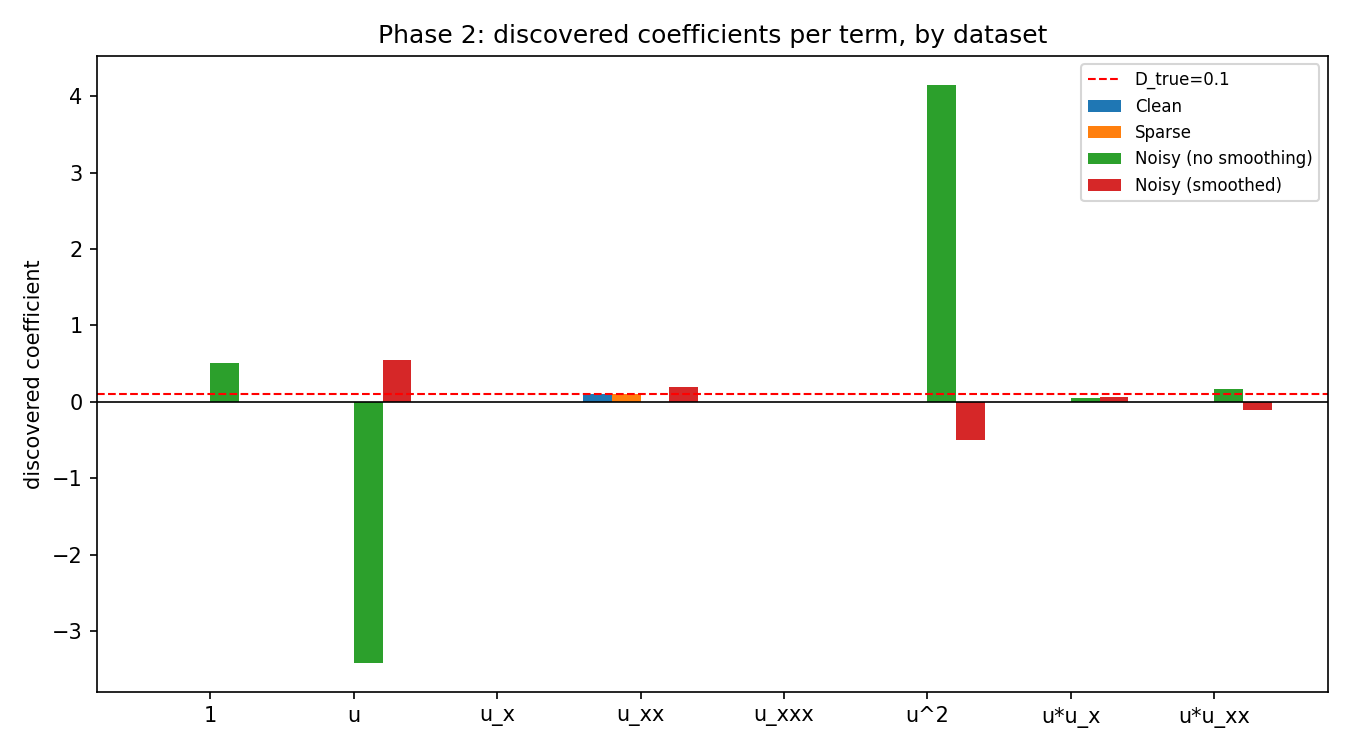
\includegraphics[width=0.88\textwidth]{results/equations/phase2_coefficients.png}
\caption{Phase~2 coefficients found by STLSQ for each run (from \fn{results/equations/}). Clean and sparse data
keep only $u_{xx}$; noisy data scatters weight over spurious terms.}
\end{figure}

\begin{lesson}[: a good fit is not the right law]
Noisy SINDy produced equations with small residuals and wrong terms. Differentiating noisy data amplifies the
noise (Section~\ref{sec:background}), and regression then explains noise with extra terms. This motivates
Phase~3: test hypotheses with a method that never differentiates the data.
\end{lesson}

% =====================================================================
\section{Phase 3: physics-informed neural networks}\label{sec:p3}
% =====================================================================

\textbf{Goal.} Build one reusable PINN (Section~\ref{sec:pinn}) and use it three ways: forward (known $D$),
inverse (estimate $D$), and hypothesis validation (diffusion vs.\ advection).

\textbf{How it works.} The network \fn{PINN} maps $(x,t)\mapsto u$ with four tanh layers of 64 units. The
\emph{only} thing that changes between hypotheses is the residual function, looked up in
\fn{RESIDUAL_REGISTRY} (diffusion, advection, reaction--diffusion). All derivatives come from autograd
(\fn{compute_derivatives}). Training draws 2000 collocation points, 200 boundary and 200 initial points, runs
3000 Adam steps then 300 L-BFGS iterations, and finally scores the result against fixed thresholds.

\begin{figure}[!htb]
\centering
% flowchart 'p3' -- used by docs/Report.tex
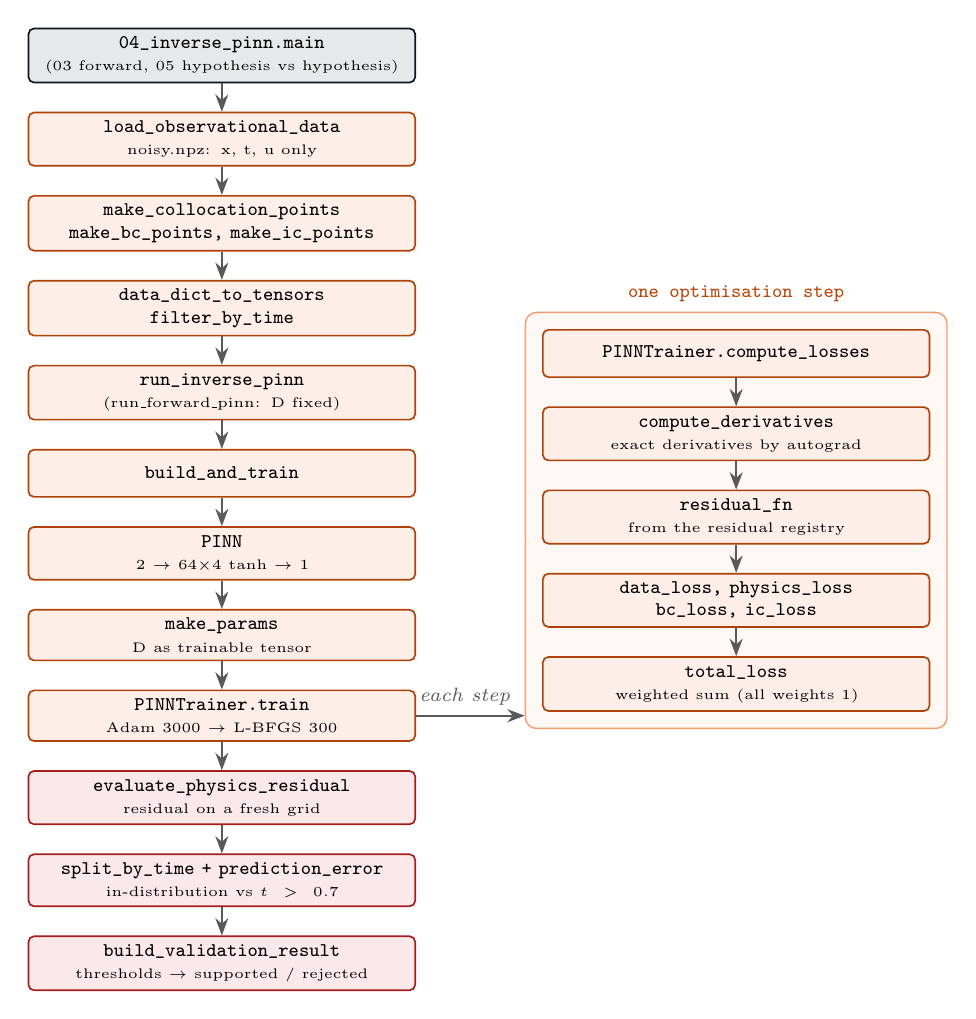
\begin{tikzpicture}[node distance=3.6mm and 6mm]
  % left column: experiment set-up
  \node[fnw=cExp] (main) {04_inverse_pinn.main\\{\normalfont\tiny (03 forward, 05 hypothesis vs hypothesis)}};
  \node[fnw=cPinn, below=of main] (load) {load_observational_data\\{\normalfont\tiny noisy.npz: x, t, u only}};
  \node[fnw=cPinn, below=of load] (pts) {make_collocation_points\\make_bc_points, make_ic_points};
  \node[fnw=cPinn, below=of pts] (tens) {data_dict_to_tensors\\filter_by_time};
  \node[fnw=cPinn, below=of tens] (inv) {run_inverse_pinn\\{\normalfont\tiny (run\_forward\_pinn: D fixed)}};
  \node[fnw=cPinn, below=of inv] (bt) {build_and_train};
  \node[fnw=cPinn, below=of bt] (net) {PINN\\{\normalfont\tiny 2 $\to$ 64$\times$4 tanh $\to$ 1}};
  \node[fnw=cPinn, below=of net] (mp) {make_params\\{\normalfont\tiny D as trainable tensor}};
  \node[fnw=cPinn, below=of mp] (tr) {PINNTrainer.train\\{\normalfont\tiny Adam 3000 $\to$ L-BFGS 300}};
  % right column: one loss evaluation
  \node[fnw=cPinn, right=of tr, xshift=10mm, yshift=46mm] (cl) {PINNTrainer.compute_losses};
  \node[fnw=cPinn, below=of cl] (cd) {compute_derivatives\\{\normalfont\tiny exact derivatives by autograd}};
  \node[fnw=cPinn, below=of cd] (res) {residual_fn\\{\normalfont\tiny from the residual registry}};
  \node[fnw=cPinn, below=of res] (loss) {data_loss, physics_loss\\bc_loss, ic_loss};
  \node[fnw=cPinn, below=of loss] (tot) {total_loss\\{\normalfont\tiny weighted sum (all weights 1)}};
  \begin{scope}[on background layer]
    \node[pkgbox=cPinn, fit=(cl)(cd)(res)(loss)(tot), label={[pkglabel=cPinn]above:one optimisation step}] (box) {};
  \end{scope}
  % scoring
  \node[fnw=cVal, below=of tr] (phys) {evaluate_physics_residual\\{\normalfont\tiny residual on a fresh grid}};
  \node[fnw=cVal, below=of phys] (ood) {split_by_time + prediction_error\\{\normalfont\tiny in-distribution vs $t>0.7$}};
  \node[fnw=cVal, below=of ood] (score) {build_validation_result\\{\normalfont\tiny thresholds $\to$ supported / rejected}};
  \foreach \a/\b in {main/load,load/pts,pts/tens,tens/inv,inv/bt,bt/net,net/mp,mp/tr,tr/phys,phys/ood,ood/score}
    \draw[flow] (\a) -- (\b);
  \draw[flow] (tr.east) -- (box.west |- tr.east) node[note, above, pos=0.45]{each step};
  \draw[flow] (cl) -- (cd); \draw[flow] (cd) -- (res); \draw[flow] (res) -- (loss); \draw[flow] (loss) -- (tot);
\end{tikzpicture}

\pkglegend
\caption{Phase~3 function flow. Left: an experiment builds tensors, creates the network and trains it. Right: what
happens inside every optimisation step. Bottom: scoring with fixed thresholds.}
\label{fig:p3}
\end{figure}

\textbf{Results.}
\begin{itemize}
  \item \textbf{Forward} ($D=0.1$ known): the PINN's prediction differs from the clean field by RMSE
        $0.000727$, even though it was trained on data with $\approx0.0116$ noise. The physics term denoises.
  \item \textbf{Inverse} ($D$ unknown, started at 0.2): $\hat D = 0.09989$, a 0.11\% error. $D$ slides from 0.2
        to 0.1 within about 1500 Adam steps and stays there.
  \item \textbf{Validation}, both trained on $t\le0.7$ only with their parameter trainable:
\end{itemize}
\begin{center}
\small
\begin{tabular}{@{}lllllll@{}}
\toprule
\textbf{Hypothesis} & \textbf{Status} & \textbf{Data loss} & \textbf{Physics} & \textbf{IC loss} & \textbf{In-dist.\ RMSE} & \textbf{OOD RMSE} \\ \midrule
H1 diffusion & supported & 0.00013 & 0.00008 & 0.000001 & 0.00078 & 0.00115 \\
H2 advection & rejected  & 0.03775 & 0.00499 & 0.02515  & 0.20033 & 0.33145 \\
\bottomrule
\end{tabular}
\end{center}
Diffusion wins on every metric by 30--290$\times$. Advection simply cannot turn a decaying double hump into
anything consistent with the data: its IC loss alone is 25{,}000 times worse.

\begin{figure}[!htb]
\centering
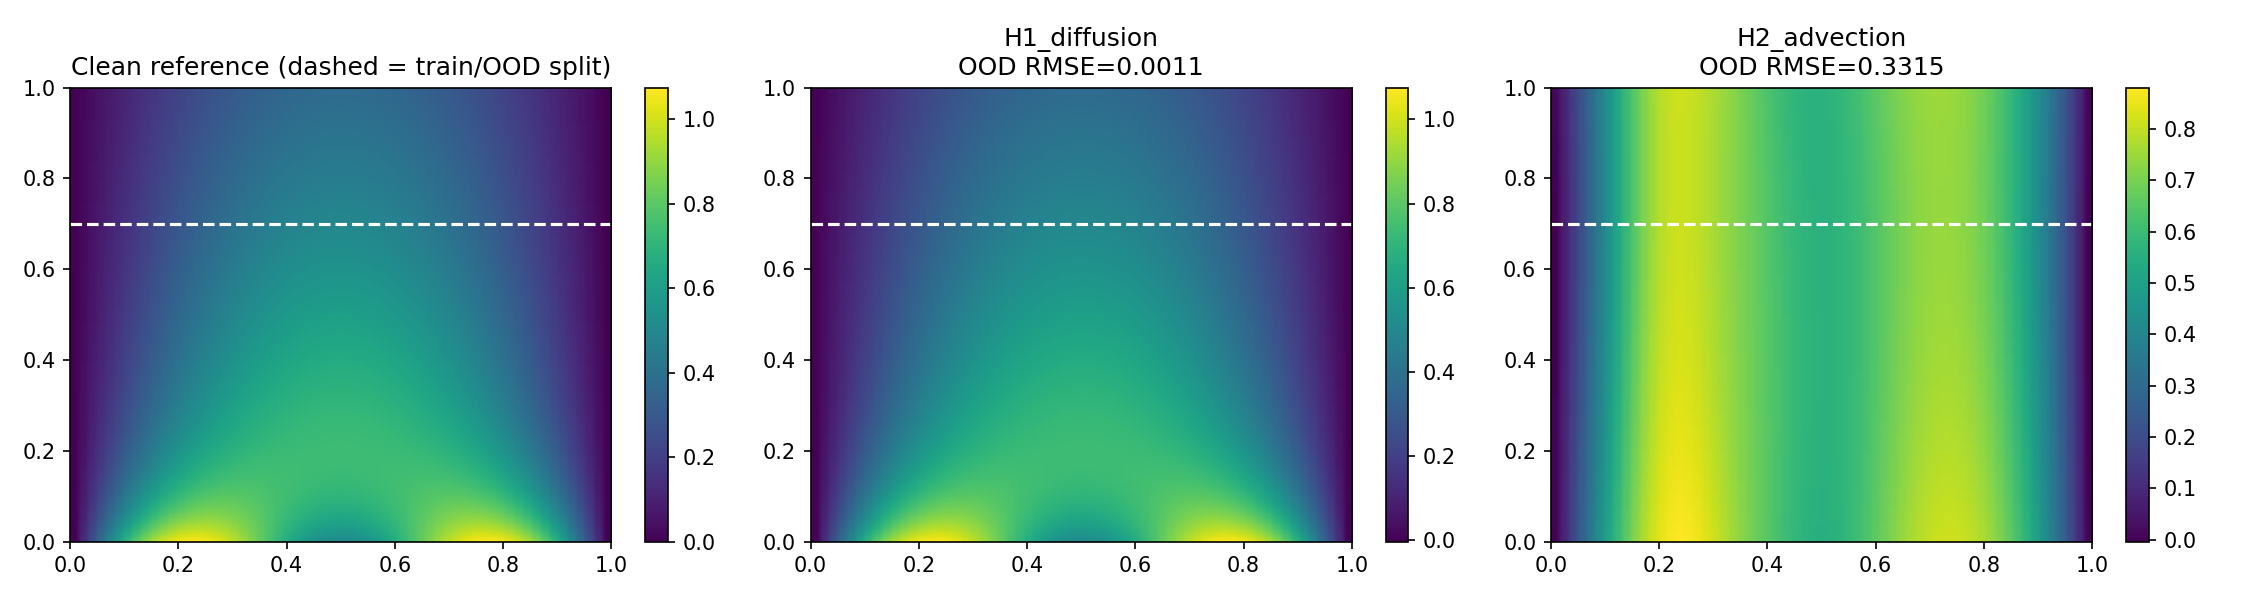
\includegraphics[width=0.92\textwidth]{results/pinn/phase3_ood_comparison.png}
\caption{Phase~3 hypothesis validation (from \fn{results/pinn/}). Training used only $t\le0.7$ (dashed line).
Diffusion reproduces the field on both sides of the split; advection converges to a wrong, roughly static
pattern.}
\end{figure}

\begin{caution}[: an audit note added in Phase 6]
The Phase~3 accept/reject rule included one check against the clean truth field. Training never used it, but a
decision did. Re-checking showed no outcome depended on it (H2 also fails its data and IC losses). Phase~6
removed the issue: from then on, decisions use only held-out \emph{noisy} observations.
\end{caution}

% =====================================================================
\section{Phase 4: generating hypotheses with an LLM}\label{sec:p4}
% =====================================================================

\textbf{Goal.} Until now a human typed each candidate equation into the code. Phase~4 adds a generator that
proposes \emph{which} equations are worth testing, from a description of what was observed, without being told
the answer. The rule that makes this safe: \emph{LLM = hypothesis generator, PINN = validator.}

\textbf{The description the LLM sees.} \fn{build_problem_description} computes only statistics of the noisy
observations and turns them into text. For the Phase~1 data it says, among other things: the peak amplitude is
about 0.983 near $t=0.05$ and about 0.395 near $t=0.95$ (``decreased substantially''); the field stays near
zero at the edges; and the centroid moves only from $x\approx0.53$ to $0.41$ (``little evidence of bulk
translation''). It never names a mechanism.

\textbf{The key design choice: a generic equation compiler.} Phase~3 needed a hand-written Python function per
equation. That does not scale to whatever an LLM might propose. \fn{compile_residual} instead parses the
equation \emph{string} with SymPy (a symbolic-maths library) and compiles it into exactly the residual function
the Phase~3 trainer expects. For example, from \texttt{"u\_t = D*u\_xx + r*u*(1-u/K)"} it detects the fields
$u, u_t, u_{xx}$ and the parameters $D, r, K$ automatically. Any combination of $u, u_t, u_x, u_{xx}, u_{xxx}$
and named parameters works with zero code changes.

\textbf{Deterministic checks before any training} (\fn{validate_hypothesis}):
\begin{enumerate}
  \item \emph{Syntax}: can SymPy parse the equation?
  \item \emph{Variables}: is $u$ the dependent variable and are $x, t$ the independent ones?
  \item \emph{Parameters}: does every symbol used appear in the declared parameter list, and vice versa?
  \item \emph{Derivatives}: do the LLM's stated \fn{required_derivatives} match what SymPy finds?
  \item \emph{Units}: what fraction of parameters declare units (reported, not a proof)?
  \item \emph{Duplicates}: \fn{canonical_signature} replaces every parameter by a placeholder and ignores sign
        and side, so \texttt{u\_t = D*u\_xx} and \texttt{k*u\_xx = u\_t} are recognised as the same equation.
\end{enumerate}

\begin{figure}[!htb]
\centering
% flowchart 'p4' -- shared by project_guide.tex and submission_report.tex
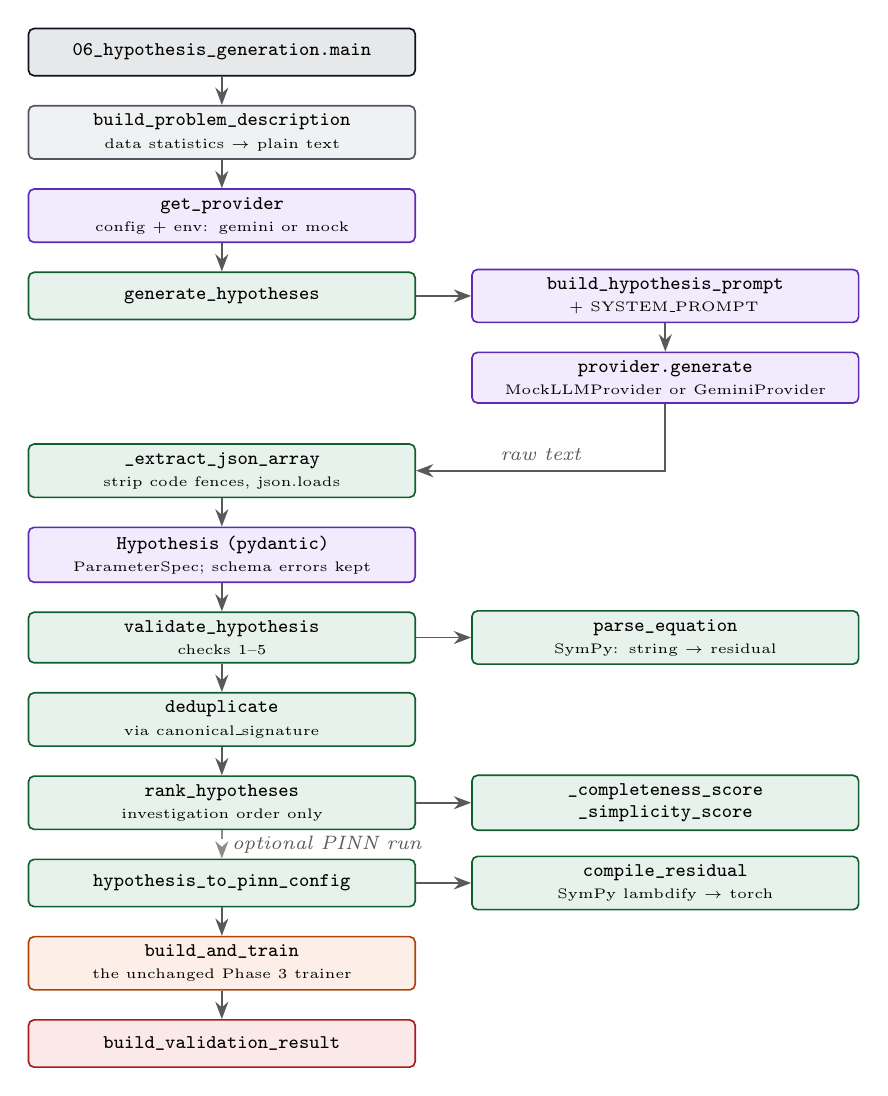
\begin{tikzpicture}[node distance=3.6mm and 7mm]
  \node[fnw=cExp] (main) {06_hypothesis_generation.main};
  \node[fnw=cData, below=of main] (desc) {build_problem_description\\{\normalfont\tiny data statistics $\to$ plain text}};
  \node[fnw=cLlm, below=of desc] (gp) {get_provider\\{\normalfont\tiny config + env: gemini or mock}};
  \node[fnw=cHyp, below=of gp] (gen) {generate_hypotheses};
  \node[fnw=cLlm, right=of gen] (prompt) {build_hypothesis_prompt\\{\normalfont\tiny + SYSTEM\_PROMPT}};
  \node[fnw=cLlm, below=of prompt] (call) {provider.generate\\{\normalfont\tiny MockLLMProvider or GeminiProvider}};
  \node[fnw=cHyp, below=of gen, yshift=-12mm] (json) {_extract_json_array\\{\normalfont\tiny strip code fences, json.loads}};
  \node[fnw=cLlm, below=of json] (schema) {Hypothesis (pydantic)\\{\normalfont\tiny ParameterSpec; schema errors kept}};
  \node[fnw=cHyp, below=of schema] (val) {validate_hypothesis\\{\normalfont\tiny checks 1--5}};
  \node[fnw=cHyp, right=of val] (parse) {parse_equation\\{\normalfont\tiny SymPy: string $\to$ residual}};
  \node[fnw=cHyp, below=of val] (dedup) {deduplicate\\{\normalfont\tiny via canonical\_signature}};
  \node[fnw=cHyp, below=of dedup] (rank) {rank_hypotheses\\{\normalfont\tiny investigation order only}};
  \node[fnw=cHyp, right=of rank] (scores) {_completeness_score\\_simplicity_score};
  \node[fnw=cHyp, below=of rank] (adapt) {hypothesis_to_pinn_config};
  \node[fnw=cHyp, right=of adapt] (comp) {compile_residual\\{\normalfont\tiny SymPy lambdify $\to$ torch}};
  \node[fnw=cPinn, below=of adapt] (train) {build_and_train\\{\normalfont\tiny the unchanged Phase 3 trainer}};
  \node[fnw=cVal, below=of train] (score) {build_validation_result};
  \draw[flow] (main) -- (desc); \draw[flow] (desc) -- (gp); \draw[flow] (gp) -- (gen);
  \draw[flow] (gen) -- (prompt); \draw[flow] (prompt) -- (call);
  \draw[flow] (call) |- node[note, above, pos=0.75]{raw text} (json);
  \draw[flow] (json) -- (schema); \draw[flow] (schema) -- (val); \draw[flow] (val) -- (parse);
  \draw[flow] (val) -- (dedup); \draw[flow] (dedup) -- (rank); \draw[flow] (rank) -- (scores);
  \draw[dflow] (rank) -- node[note, right]{optional PINN run} (adapt);
  \draw[flow] (adapt) -- (comp); \draw[flow] (adapt) -- (train); \draw[flow] (train) -- (score);
\end{tikzpicture}

\pkglegend
\caption{Phase~4 function flow: describe $\to$ prompt $\to$ LLM $\to$ parse JSON $\to$ schema $\to$ deterministic
checks $\to$ deduplicate $\to$ rank $\to$ (optionally) compile into a PINN and validate.}
\label{fig:p4}
\end{figure}

\textbf{Results (mock LLM, all four candidates run through the Phase~3 PINN).}
\begin{center}
\small
\begin{tabular}{@{}llll@{}}
\toprule
\textbf{ID} & \textbf{Equation} & \textbf{PINN status} & \textbf{Fitted parameters} \\ \midrule
H1 & $u_t = D\,u_{xx}$ & supported & $D=0.09989$ \\
H2 & $u_t + c\,u_x = 0$ & rejected & $c=0.0164$ \\
H3 & $u_t = D\,u_{xx} + r\,u(1-u/K)$ & supported & $D=0.1006,\ r=0.0148,\ K=1.215$ \\
H4 & $u_t + c\,u_x = D\,u_{xx}$ & supported & $c=-0.0004,\ D=0.0999$ \\
\bottomrule
\end{tabular}
\end{center}

\begin{lesson}[: validation alone cannot reject harmless extra terms]
H3 and H4 \emph{contain} diffusion as a special case. Their extra parameters converged to almost exactly the
``switch this term off'' values ($r\approx0.015$, $c\approx0$), so they fit as well as H1 and pass the same
thresholds. A pass/fail validator cannot tell ``minimal correct model'' from ``needlessly general model that
also fits''. This is the \textbf{nested-model problem} (Section~\ref{sec:selection}), and it is why Phase~6 adds
term necessity, complexity and BIC to the selection.
\end{lesson}

% =====================================================================
\section{Phase 5: scientific RAG and a knowledge graph}\label{sec:p5}
% =====================================================================

\textbf{Goal.} Ground hypothesis generation in retrieved scientific evidence (RAG), and organise that evidence as
a knowledge graph with provenance, so every fact can be traced to its source.

\textbf{The corpus.} Five short Markdown documents in \fn{rag/corpus/}: diffusion, advection, reaction,
reaction--diffusion and advection--diffusion. Each has a front-matter header (id, title, source, domain,
declared mechanism, declared equations, declared parameters) and textbook-style sections.

\textbf{Preventing answer leakage.} Documents state only the generic textbook law (e.g.\ ``Fick's second law,
$u_t=D\,u_{xx}$''). They never state this dataset's $D=0.1$ and never say ``this data is diffusion''. A real
scientist knows the textbook candidates before looking at new data; knowing the answer would be cheating. An
automated check confirms the string ``0.1'' appears in no corpus document.

\begin{figure}[!htb]
\centering
% flowchart 'p5' -- shared by project_guide.tex and submission_report.tex
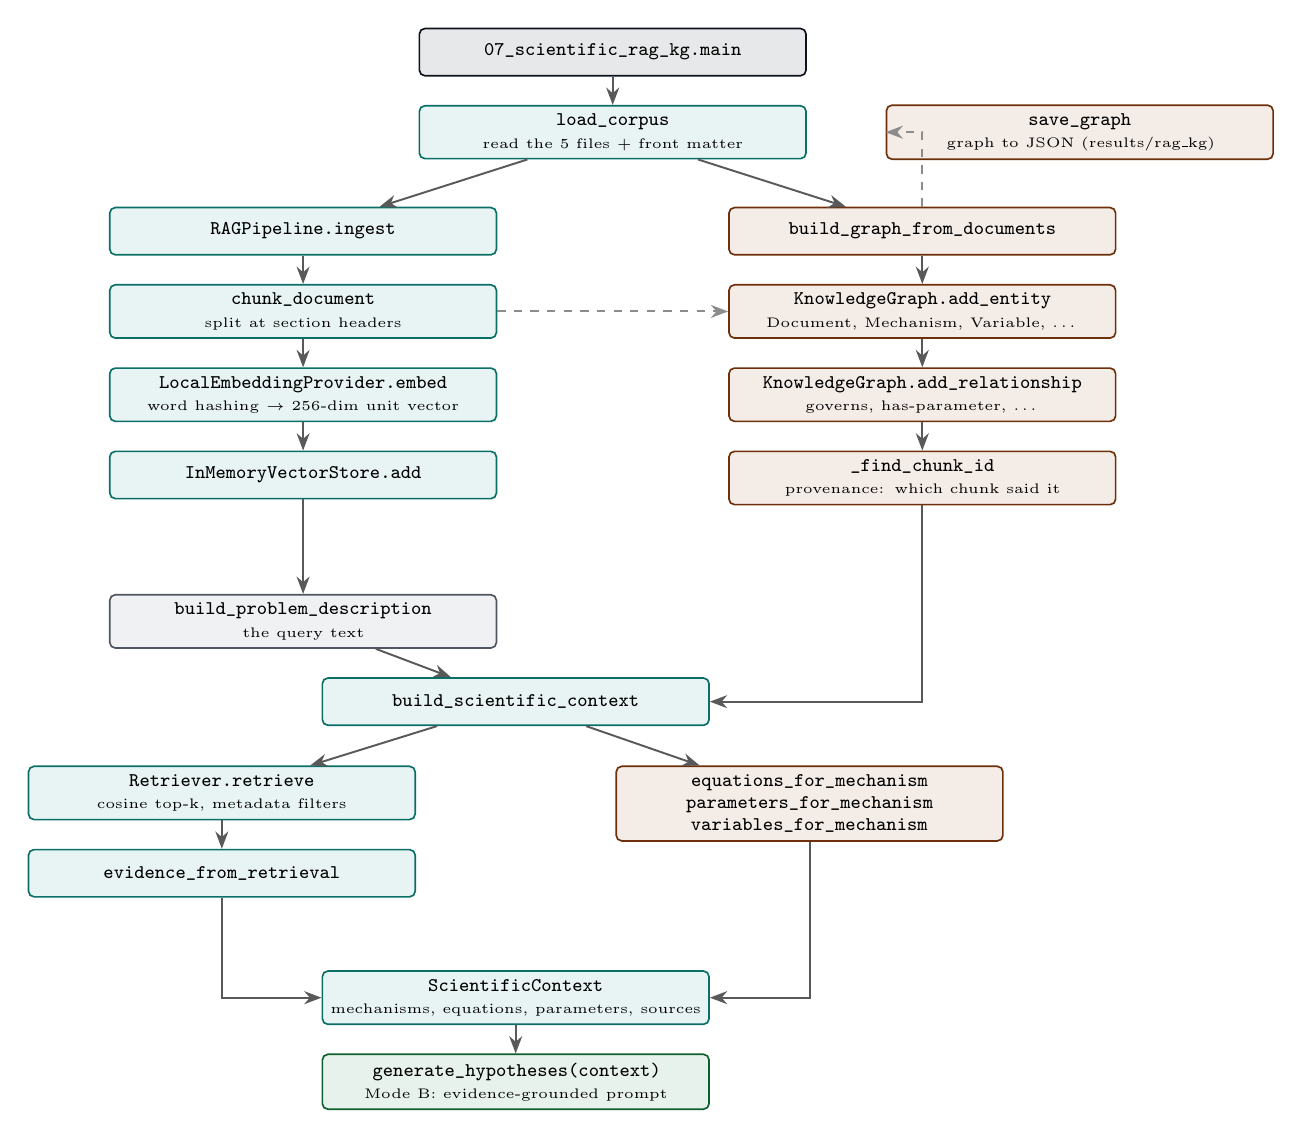
\begin{tikzpicture}[node distance=3.6mm and 6mm]
  \node[fnw=cExp] (main) {07_scientific_rag_kg.main};
  \node[fnw=cRag, below=of main] (lc) {load_corpus\\{\normalfont\tiny read the 5 files + front matter}};
  % RAG column (left)
  \node[fnw=cRag, below left=6mm and -10mm of lc] (ing) {RAGPipeline.ingest};
  \node[fnw=cRag, below=of ing] (chunk) {chunk_document\\{\normalfont\tiny split at section headers}};
  \node[fnw=cRag, below=of chunk] (emb) {LocalEmbeddingProvider.embed\\{\normalfont\tiny word hashing $\to$ 256-dim unit vector}};
  \node[fnw=cRag, below=of emb] (vs) {InMemoryVectorStore.add};
  % KG column (right)
  \node[fnw=cKg, below right=6mm and -10mm of lc] (bg) {build_graph_from_documents};
  \node[fnw=cKg, below=of bg] (ent) {KnowledgeGraph.add_entity\\{\normalfont\tiny Document, Mechanism, Variable, \ldots}};
  \node[fnw=cKg, below=of ent] (rel) {KnowledgeGraph.add_relationship\\{\normalfont\tiny governs, has-parameter, \ldots}};
  \node[fnw=cKg, below=of rel] (src) {_find_chunk_id\\{\normalfont\tiny provenance: which chunk said it}};
  % merge
  \node[fnw=cData, below=12mm of vs] (pd) {build_problem_description\\{\normalfont\tiny the query text}};
  \node[fnw=cRag, below=of pd, xshift=27mm] (ctx) {build_scientific_context};
  \node[fnw=cRag, below left=5mm and -12mm of ctx] (ret) {Retriever.retrieve\\{\normalfont\tiny cosine top-k, metadata filters}};
  \node[fnw=cRag, below=of ret] (ev) {evidence_from_retrieval};
  \node[fnw=cKg, below right=5mm and -12mm of ctx] (q) {equations_for_mechanism\\parameters_for_mechanism\\variables_for_mechanism};
  \node[fnw=cRag, below=31mm of ctx] (sc) {ScientificContext\\{\normalfont\tiny mechanisms, equations, parameters, sources}};
  \node[fnw=cHyp, below=of sc] (gen) {generate_hypotheses(context)\\{\normalfont\tiny Mode B: evidence-grounded prompt}};
  \node[fnw=cKg, right=of lc, xshift=4mm] (ser) {save_graph\\{\normalfont\tiny graph to JSON (results/rag\_kg)}};
  \draw[flow] (main) -- (lc); \draw[flow] (lc) -- (ing); \draw[flow] (lc) -- (bg);
  \draw[flow] (ing) -- (chunk); \draw[flow] (chunk) -- (emb); \draw[flow] (emb) -- (vs);
  \draw[flow] (bg) -- (ent); \draw[flow] (ent) -- (rel); \draw[flow] (rel) -- (src);
  \draw[dflow] (chunk.east) -- (bg.west |- chunk.east);
  \draw[dflow] (bg.north) |- (ser.west);
  \draw[flow] (vs) -- (pd); \draw[flow] (pd) -- (ctx); \draw[flow] (src) |- (ctx);
  \draw[flow] (ctx) -- (ret); \draw[flow] (ret) -- (ev); \draw[flow] (ctx) -- (q);
  \draw[flow] (ev) |- (sc); \draw[flow] (q) |- (sc); \draw[flow] (sc) -- (gen);
\end{tikzpicture}

\pkglegend
\caption{Phase~5 function flow. Left: RAG indexing (chunk, embed, store). Right: knowledge-graph construction
with provenance (the dashed arrow: chunks give each relationship its source). Bottom: the observation
description is used as a query; retrieved evidence and graph queries merge into one \fn{ScientificContext} that
is passed to the hypothesis generator.}
\label{fig:p5}
\end{figure}

\textbf{Results.}
\begin{itemize}
  \item The graph has \textbf{22 entities} (5 documents, 5 mechanisms, 3 variables, 4 parameters, 5 equations)
        and \textbf{40 relationships, all sourced}. Shared concepts merge: there is a single node for $D$,
        even though three documents declare it, and repeated facts merge their sources instead of creating
        duplicate edges.
  \item Example queries: asking \fn{equations_for_mechanism} about diffusion returns \texttt{u\_t = D*u\_xx},
        and asking \fn{parameters_for_mechanism} returns \texttt{D}.
  \item For the Phase~1 data, the context contained the mechanisms advection, diffusion and reaction, their
        three textbook equations, and the parameters $D, K, c, r$.
  \item \textbf{Mode A} (no context) and \textbf{Mode B} (with context) produced the identical four candidate equations. That is
        expected: the mock LLM returns canned answers whatever the prompt. Showing that evidence changes the
        proposals needs a real LLM (Section~\ref{sec:gemini}).
\end{itemize}

\begin{lesson}[: RAG and the graph do different jobs]
RAG answers ``which text is relevant?'' by similarity; it is fuzzy and ranked. The graph answers ``how are these
documented concepts related, and who said so?''; it is exact and traceable. Neither decides what is true.
Phase~7 measures their real contribution and finds it modest: RAG gives 100\% recall of the right mechanism on a
5-document corpus, but top-1 retrieval is right only 1 time in 6.
\end{lesson}

% =====================================================================
\section{Phase 6: the physics-constrained generative search}\label{sec:p6}
% =====================================================================

\textbf{Goal.} Assemble everything into one honest discovery pipeline (Figure~\ref{fig:pipeline}) that searches
over candidate equations, tests each with an inverse PINN, and selects the most parsimonious supported law,
\emph{without the truth influencing any decision}.

\textbf{Three stages.} Each inverse PINN takes about 4 minutes on a CPU, so the experiment runs in stages and
caches every candidate. The script is \fn{experiments/08_physics_constrained_search.py}:
\begin{enumerate}
  \item \fn{stage_prepare}: RAG, graph, context, LLM generation, knowledge-graph templates, deduplication,
        structural and physics pre-checks. No training.
  \item \fn{stage_pinn}: one inverse PINN per surviving candidate, on the training split only.
  \item \fn{stage_select}: stability, model selection, baselines, OOD and novel prediction, then the oracle
        report and plots.
\end{enumerate}

\textbf{The splits.} Train on $t\le0.8$ (minus a random 20\% holdout); gate and select on that holdout; test
extrapolation on all $t>0.8$ points, which no decision ever sees. Collocation, BC and IC points are also
restricted to $t\le0.8$, so OOD prediction is genuine extrapolation.

\textbf{Physics constraints.} Each parameter can carry bounds; \fn{config.yaml} supplies fallbacks $D>0$ and
$K>0$ ($c$ and $r$ may have either sign). Before training, \fn{precheck_physics} rejects non-evolution equations
and warns on two real modelling issues: advection with fixed values at both ends is over-determined, and an
equation with no spatial derivative cannot interact with boundary conditions at all.

\begin{figure}[p]
\centering
% flowchart 'p6' -- shared by project_guide.tex and submission_report.tex
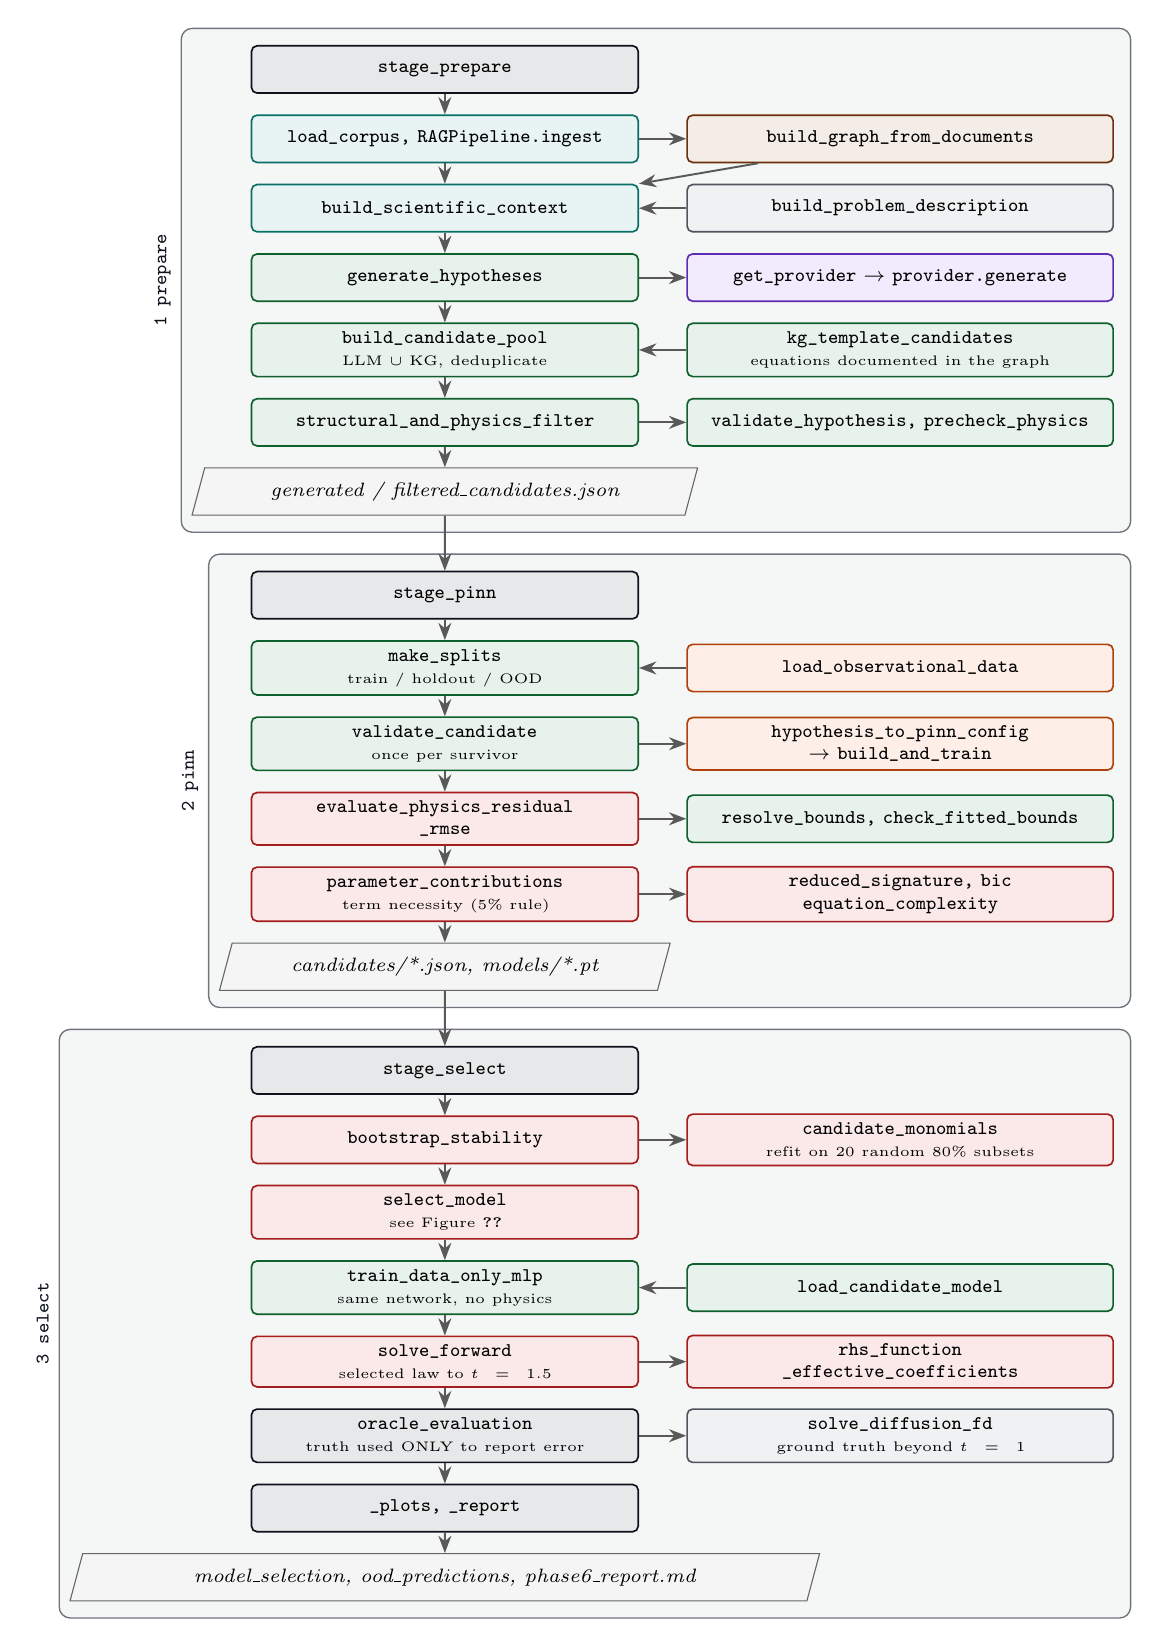
\begin{tikzpicture}[node distance=2.6mm and 6mm]
  \tikzset{sp/.style={fnw=#1}, hp/.style={fnw=#1, text width=52mm}}
  % ---------------- stage 1 ----------------
  \node[sp=cExp] (p0) {stage_prepare};
  \node[sp=cRag, below=of p0] (p1) {load_corpus, RAGPipeline.ingest};
  \node[hp=cKg, right=of p1] (h1) {build_graph_from_documents};
  \node[sp=cRag, below=of p1] (p2) {build_scientific_context};
  \node[hp=cData, right=of p2] (h2) {build_problem_description};
  \node[sp=cHyp, below=of p2] (p3) {generate_hypotheses};
  \node[hp=cLlm, right=of p3] (h3) {get_provider $\to$ provider.generate};
  \node[sp=cHyp, below=of p3] (p4) {build_candidate_pool\\{\normalfont\tiny LLM $\cup$ KG, deduplicate}};
  \node[hp=cHyp, right=of p4] (h4) {kg_template_candidates\\{\normalfont\tiny equations documented in the graph}};
  \node[sp=cHyp, below=of p4] (p5) {structural_and_physics_filter};
  \node[hp=cHyp, right=of p5] (h5) {validate_hypothesis, precheck_physics};
  \node[io, below=of p5] (o1) {generated / filtered\_candidates.json};
  % ---------------- stage 2 ----------------
  \node[sp=cExp, below=7mm of o1] (q0) {stage_pinn};
  \node[sp=cHyp, below=of q0] (q1) {make_splits\\{\normalfont\tiny train / holdout / OOD}};
  \node[hp=cPinn, right=of q1] (g1) {load_observational_data};
  \node[sp=cHyp, below=of q1] (q2) {validate_candidate\\{\normalfont\tiny once per survivor}};
  \node[hp=cPinn, right=of q2] (g2) {hypothesis_to_pinn_config\\$\to$ build_and_train};
  \node[sp=cVal, below=of q2] (q3) {evaluate_physics_residual\\_rmse};
  \node[hp=cHyp, right=of q3] (g3) {resolve_bounds, check_fitted_bounds};
  \node[sp=cVal, below=of q3] (q4) {parameter_contributions\\{\normalfont\tiny term necessity (5\% rule)}};
  \node[hp=cVal, right=of q4] (g4) {reduced_signature, bic\\equation_complexity};
  \node[io, below=of q4] (o2) {candidates/*.json, models/*.pt};
  % ---------------- stage 3 ----------------
  \node[sp=cExp, below=7mm of o2] (r0) {stage_select};
  \node[sp=cVal, below=of r0] (r1) {bootstrap_stability};
  \node[hp=cVal, right=of r1] (k1) {candidate_monomials\\{\normalfont\tiny refit on 20 random 80\% subsets}};
  \node[sp=cVal, below=of r1] (r2) {select_model\\{\normalfont\tiny see Figure \ref{fig:selection}}};
  \node[sp=cHyp, below=of r2] (r3) {train_data_only_mlp\\{\normalfont\tiny same network, no physics}};
  \node[hp=cHyp, right=of r3] (k3) {load_candidate_model};
  \node[sp=cVal, below=of r3] (r4) {solve_forward\\{\normalfont\tiny selected law to $t=1.5$}};
  \node[hp=cVal, right=of r4] (k4) {rhs_function\\_effective_coefficients};
  \node[sp=cExp, below=of r4] (r5) {oracle_evaluation\\{\normalfont\tiny truth used ONLY to report error}};
  \node[hp=cData, right=of r5] (k5) {solve_diffusion_fd\\{\normalfont\tiny ground truth beyond $t=1$}};
  \node[sp=cExp, below=of r5] (r6) {_plots, _report};
  \node[io, below=of r6] (o3) {model\_selection, ood\_predictions, phase6\_report.md};
  % groups
  \begin{scope}[on background layer]
    \node[pkgbox=cExp, fit=(p0)(h1)(h5)(o1), label={[pkglabel=cExp]left:\rotatebox{90}{1 prepare}}] {};
    \node[pkgbox=cExp, fit=(q0)(g1)(g4)(o2), label={[pkglabel=cExp]left:\rotatebox{90}{2 pinn}}] {};
    \node[pkgbox=cExp, fit=(r0)(k1)(k5)(o3), label={[pkglabel=cExp]left:\rotatebox{90}{3 select}}] {};
  \end{scope}
  % arrows
  \foreach \a/\b in {p0/p1,p1/p2,p2/p3,p3/p4,p4/p5,p5/o1,o1/q0,q0/q1,q1/q2,q2/q3,q3/q4,q4/o2,o2/r0,r0/r1,r1/r2,r2/r3,r3/r4,r4/r5,r5/r6,r6/o3}
    \draw[flow] (\a) -- (\b);
  \foreach \a/\b in {p1/h1,h2/p2,p3/h3,h4/p4,p5/h5,g1/q1,q2/g2,q3/g3,q4/g4,r1/k1,k3/r3,r4/k4,r5/k5}
    \draw[flow] (\a) -- (\b);
  \draw[flow] (h1) -- (p2.north east);
\end{tikzpicture}

\pkglegend
\caption{Phase~6 function flow, stage by stage. The left spine is the order of execution; the right column holds
the helper functions each step calls. Only \fn{oracle_evaluation} ever touches the ground truth, and it runs
after every decision is made.}
\label{fig:p6}
\end{figure}

\begin{figure}[!htb]
\centering
% flowchart 'selection' -- used by docs/Report.tex
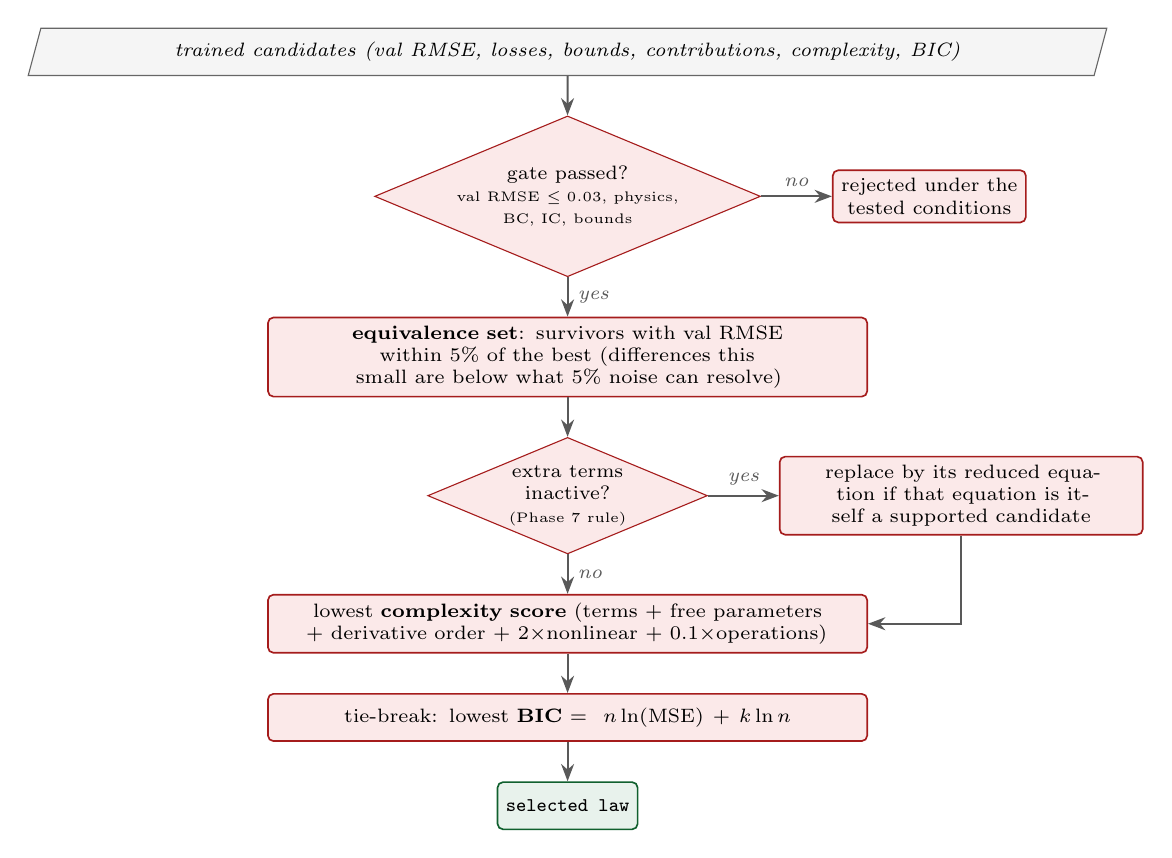
\begin{tikzpicture}[node distance=5mm and 9mm]
  \node[io] (in) {trained candidates (val RMSE, losses, bounds, contributions, complexity, BIC)};
  \node[dec=cVal, below=of in] (g) {gate passed?\\{\tiny val RMSE $\le 0.03$, physics,}\\{\tiny BC, IC, bounds}};
  \node[fn=cVal, font=\scriptsize, right=of g] (rej) {rejected under the\\tested conditions};
  \node[fn=cVal, font=\scriptsize, below=of g, text width=74mm] (eq) {\textbf{equivalence set}: survivors with val RMSE within 5\% of the best
        (differences this small are below what 5\% noise can resolve)};
  \node[dec=cVal, below=of eq] (red) {extra terms\\inactive?\\{\tiny (Phase 7 rule)}};
  \node[fn=cVal, font=\scriptsize, right=of red, text width=44mm] (rd) {replace by its reduced equation if that equation is
        itself a supported candidate};
  \node[fn=cVal, font=\scriptsize, below=of red, text width=74mm] (cx) {lowest \textbf{complexity score}
        (terms + free parameters + derivative order + 2$\times$nonlinear + 0.1$\times$operations)};
  \node[fn=cVal, font=\scriptsize, below=of cx, text width=74mm] (bic) {tie-break: lowest \textbf{BIC} $= n\ln(\mathrm{MSE}) + k\ln n$};
  \node[fn=cHyp, below=of bic] (sel) {\textbf{selected law}};
  \draw[flow] (in) -- (g);
  \draw[flow] (g) -- node[note, above]{no} (rej);
  \draw[flow] (g) -- node[note, right]{yes} (eq);
  \draw[flow] (eq) -- (red);
  \draw[flow] (red) -- node[note, above]{yes} (rd);
  \draw[flow] (rd) |- (cx.east);
  \draw[flow] (red) -- node[note, right]{no} (cx);
  \draw[flow] (cx) -- (bic); \draw[flow] (bic) -- (sel);
\end{tikzpicture}

\caption{The selection rule inside \fn{select_model}, with thresholds fixed in \fn{config.yaml} before any run.
The ``inactive terms'' step is the opt-in Phase~7 refinement (\fn{prefer_reduced}); Phase~6 used only the
term-necessity numbers to \emph{explain} its choice.}
\label{fig:selection}
\end{figure}

\textbf{Results (mock LLM).} The pool held four LLM candidates plus the graph templates. The graph's diffusion and
advection templates were recognised as duplicates of H1 and H2, but the graph contributed one genuinely new
candidate the LLM had not proposed: pure reaction (K3).

\begin{center}
\footnotesize\setlength{\tabcolsep}{4pt}
\begin{tabular}{@{}llllll@{}}
\toprule
\textbf{ID} & \textbf{Equation} & \textbf{Estimates} & \textbf{Holdout RMSE} & \textbf{Status} & \textbf{Inactive} \\ \midrule
H1 & $u_t = D\,u_{xx}$ & $D=0.10002$ & 0.01214 & \textbf{selected} & -- \\
H2 & $u_t + c\,u_x = 0$ & $c=0.0089$ & 0.2269 & rejected & -- \\
H3 & $u_t = D\,u_{xx} + r\,u(1-u/K)$ & $D=0.101,\ r=0.023,\ K=1.18$ & 0.01217 & supported & $r, K$ \\
H4 & $u_t + c\,u_x = D\,u_{xx}$ & $c=-0.0002,\ D=0.09995$ & 0.01214 & supported & $c$ \\
K3 & $u_t = r\,u(1-u/K)$ & $r=-1.44,\ K=6.67$ & 0.1176 & rejected & -- \\
\bottomrule
\end{tabular}
\end{center}

H1, H3 and H4 all sit at the noise floor ($\approx0.012$), so they are fit-equivalent; H3 and H4 have inactive
extra terms and reduce to H1; H1 has the lowest complexity, and BIC agrees independently. Note that H4 had the
\emph{lowest raw} holdout error (by 0.06\%). A pure best-fit rule would have picked the more complex model.

\textbf{Out-of-distribution and novel prediction} (columns marked ``oracle'' are evaluation only):
\begin{center}
\small
\begin{tabular}{@{}lll@{}}
\toprule
\textbf{Model} & \textbf{OOD RMSE, noisy obs.} & \textbf{OOD RMSE, clean (oracle)} \\ \midrule
H1 PINN (selected) & 0.0114 & 0.0018 \\
H2 PINN (rejected) & 0.3249 & 0.3337 \\
Data-only MLP (no physics) & 0.0727 & 0.0712 \\
Forward solve of the selected law & 0.0113 & 0.0003 \\
\bottomrule
\end{tabular}
\end{center}
Solved forward to $t\in(1.0,1.5]$, where no data exists at all, the selected law has oracle RMSE
$2.5\times10^{-4}$. The physics-free network is about 40 times worse out of distribution.

\begin{figure}[!htb]
\centering
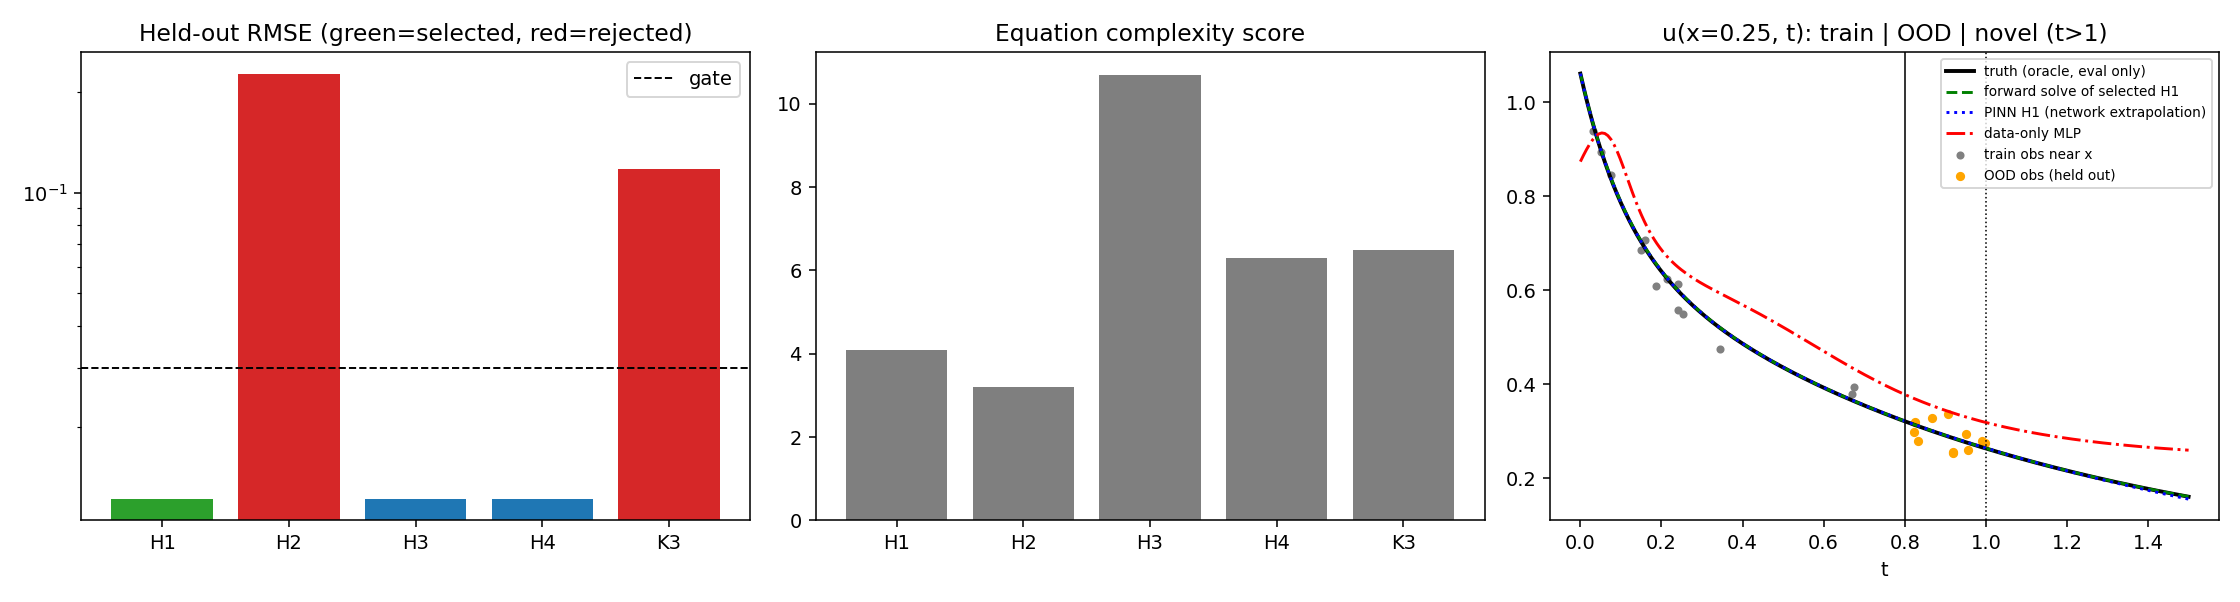
\includegraphics[width=\textwidth]{results/phase6/phase6_summary.png}
\caption{Phase~6 summary (from \fn{results/phase6/}): held-out error per candidate with the gate line (left),
complexity scores (middle), and a time trace at $x=0.25$ through train, OOD and novel windows (right).}
\end{figure}

\begin{caution}[: a disagreement reported, not hidden]
The bootstrap stability check (\fn{bootstrap_stability}) refits terms by least squares on finite-difference
derivatives, a cheap proxy, not PINN retraining and not Bayesian. For H3 it finds sign-stable $u$ and $u^2$
coefficients, while the PINN finds the reaction term contributes under 1\%. The same spurious terms appear in
Phase~2's noisy SINDy failure, which points to a finite-difference artefact. The report flags this instead of
choosing the convenient answer.
\end{caution}

% =====================================================================
\section{Phase 7: evaluation, attacks and generalisation}\label{sec:p7}
% =====================================================================

\textbf{Goal.} One success on one system proves little. Phase~7 asks: does the pipeline work across mechanism
families? Can it be fooled? Which components actually matter? Does it generalise to a new system?

\textbf{What was built} (the \fn{evaluation/} package, no new architecture):
\begin{itemize}
  \item \fn{datasets.py}: \textbf{12 benchmark datasets}, 4 families $\times$ 3 parameter settings, using exact
        analytic solutions where they exist and RK4 otherwise.
  \item \fn{describe.py}: turns any dataset into the text query for RAG with one fixed template; a test checks it
        never names a mechanism.
  \item \fn{engine.py}: the Phase~6 pipeline with the PINN swapped for fast least squares on finite-difference
        derivatives, so 95 items run in about a minute. (The PINN version runs separately on a second system.)
  \item \fn{identify.py}, \fn{benchmark.py}, \fn{adversarial.py}, \fn{ablation.py}, \fn{leakage.py}.
\end{itemize}

\begin{figure}[!htb]
\centering
% flowchart 'p7' -- shared by project_guide.tex and submission_report.tex
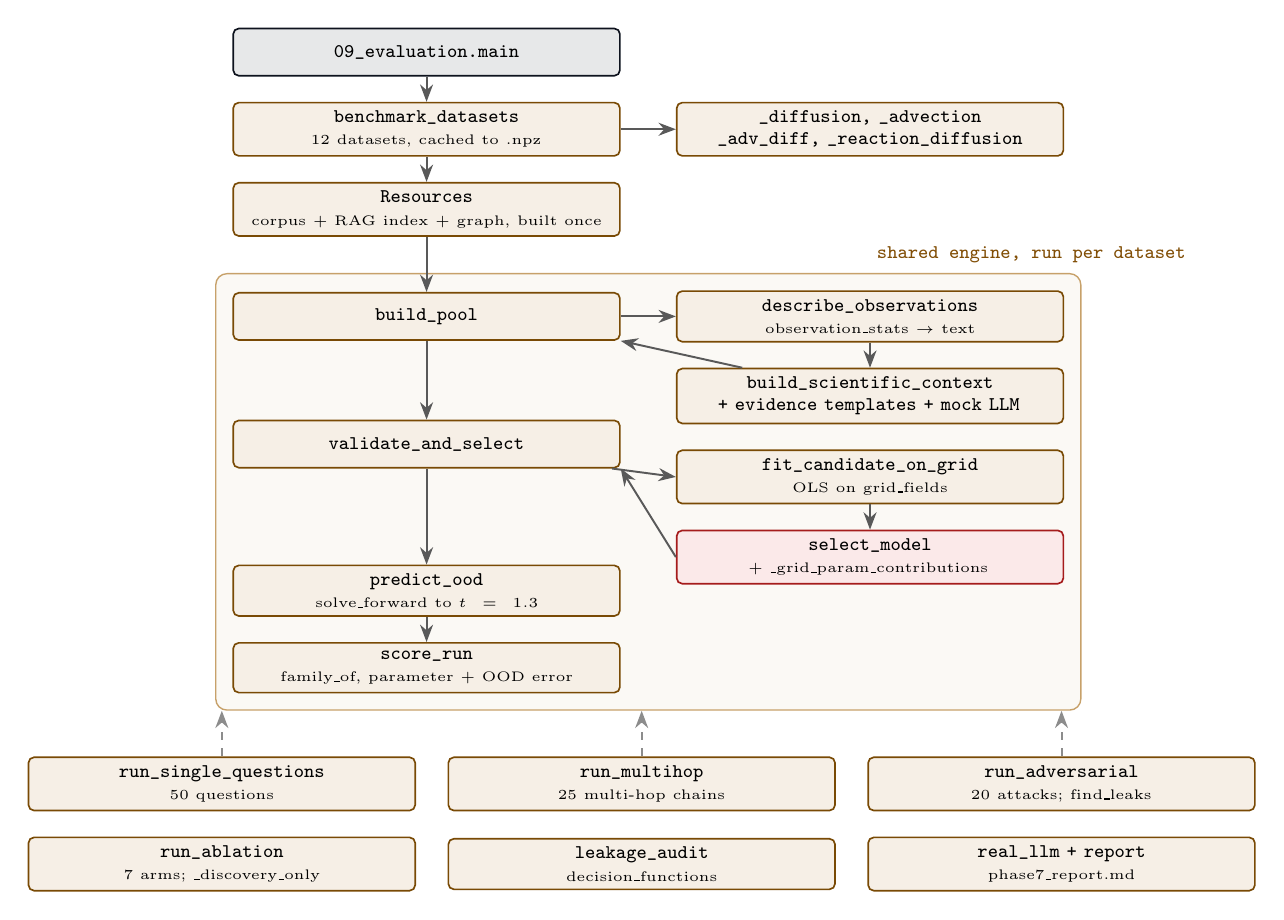
\begin{tikzpicture}[node distance=3.2mm and 7mm]
  \node[fnw=cExp] (main) {09_evaluation.main};
  \node[fnw=cEval, below=of main] (ds) {benchmark_datasets\\{\normalfont\tiny 12 datasets, cached to .npz}};
  \node[fnw=cEval, right=of ds] (mk) {_diffusion, _advection\\_adv_diff, _reaction_diffusion};
  \node[fnw=cEval, below=of ds] (res) {Resources\\{\normalfont\tiny corpus + RAG index + graph, built once}};
  \node[fnw=cEval, below=7mm of res] (bp) {build_pool};
  \node[fnw=cEval, right=of bp] (dsc) {describe_observations\\{\normalfont\tiny observation_stats $\to$ text}};
  \node[fnw=cEval, below=of dsc] (ctx) {build_scientific_context\\+ evidence templates + mock LLM};
  \node[fnw=cEval, below=10mm of bp] (vs) {validate_and_select};
  \node[fnw=cEval, below=of ctx] (fit) {fit_candidate_on_grid\\{\normalfont\tiny OLS on grid_fields}};
  \node[fnw=cVal, below=of fit] (sm) {select_model\\{\normalfont\tiny + _grid_param_contributions}};
  \node[fnw=cEval, below=of vs, yshift=-9mm] (ood) {predict_ood\\{\normalfont\tiny solve_forward to $t=1.3$}};
  \node[fnw=cEval, below=of ood] (sc) {score_run\\{\normalfont\tiny family_of, parameter + OOD error}};
  \begin{scope}[on background layer]
    \node[pkgbox=cEval, fit=(bp)(dsc)(sm)(sc), label={[pkglabel=cEval]above right:shared engine, run per dataset}] (eng) {};
  \end{scope}
  % suites
  \node[fnw=cEval, below=8mm of sc, xshift=-26mm] (s1) {run_single_questions\\{\normalfont\tiny 50 questions}};
  \node[fnw=cEval, right=4mm of s1] (s2) {run_multihop\\{\normalfont\tiny 25 multi-hop chains}};
  \node[fnw=cEval, right=4mm of s2] (s3) {run_adversarial\\{\normalfont\tiny 20 attacks; find_leaks}};
  \node[fnw=cEval, below=of s1] (s4) {run_ablation\\{\normalfont\tiny 7 arms; _discovery_only}};
  \node[fnw=cEval, right=4mm of s4] (s5) {leakage_audit\\{\normalfont\tiny decision_functions}};
  \node[fnw=cEval, right=4mm of s5] (s6) {real_llm + report\\{\normalfont\tiny phase7_report.md}};
  \draw[flow] (main) -- (ds); \draw[flow] (ds) -- (mk); \draw[flow] (ds) -- (res); \draw[flow] (res) -- (bp);
  \draw[flow] (bp) -- (dsc); \draw[flow] (dsc) -- (ctx); \draw[flow] (ctx) -- (bp.south east);
  \draw[flow] (bp) -- (vs); \draw[flow] (vs) -- (fit.west); \draw[flow] (fit) -- (sm); \draw[flow] (sm.west) -- (vs.south east);
  \draw[flow] (vs) -- (ood); \draw[flow] (ood) -- (sc);
  \draw[dflow] (s1.north) -- (s1.north |- eng.south);
  \draw[dflow] (s2.north) -- (s2.north |- eng.south);
  \draw[dflow] (s3.north) -- (s3.north |- eng.south);
\end{tikzpicture}

\pkglegend
\caption{Phase~7 function flow. A shared engine (shaded box) runs the pipeline on each benchmark dataset; the six
suites (bottom) call it in different ways. \fn{10_generalization.py} separately runs the full PINN pipeline
(\fn{validate_candidate}, \fn{select_model}) on a new system.}
\label{fig:p7}
\end{figure}

\subsection*{Results}

\textbf{50 questions: 50/50.} Structure identification 12/12, parameters within 5\% 12/12, plus graph, compiler,
complexity and retrieval-recall questions. Caveat: several categories are easy by construction, and
\textbf{top-1 retrieval is right only 1 time in 6}.

\textbf{25 multi-hop problems: 23/25.} The longest chains (data $\to$ description $\to$ RAG $\to$ graph $\to$
validation $\to$ selection $\to$ beyond-window prediction, 6 hops) score 12/12. Both failures come from top-1
lexical retrieval choosing ``advection'' for combined mechanisms.

\textbf{20 adversarial attacks: 20/20.} Examples: undeclared symbols, missing time derivative, negative
diffusivity, \emph{time-reversed data whose best fit needs $D<0$} (rejected by the physical bound), disguised
duplicates, malicious LLM output, the eigenfunction trap (flagged non-identifiable), a simpler-but-wrong
candidate on reaction--diffusion data (rejected at 85\% error rather than chosen for simplicity), corpus answer
leakage and prompt injection. Three noise/sparsity cases pass \emph{by abstention}: no candidate clears the gate,
which is safe but is not discovery.

\textbf{Ablation: which components matter?} (correct model out of 12 datasets)
\begin{center}
\small
\begin{tabular}{@{}lc@{}}
\toprule
\textbf{Arm} & \textbf{Correct} \\ \midrule
SINDy alone & 8/12 (advection--diffusion 0/3) \\
RAG + generation, no validation & 3/12 (always ``diffusion'') \\
RAG + graph + generation, no validation & 3/12 \\
\textbf{Full system} & \textbf{12/12} \\
Full system with the original Phase~6 rule & 10/12 \\
Full system without the LLM & 12/12 \\
Retrieved-evidence equations + validation (no graph, no LLM) & 12/12 \\
\bottomrule
\end{tabular}
\end{center}

\begin{lesson}[: what each part really contributes]
Physics validation and selection produce the correct answers; without them, generation just repeats its
favourite guess. RAG supplies a candidate pool that contains the truth. On this benchmark, the graph and the
\emph{mock} LLM add no measurable accuracy; the graph's value is structured querying and provenance. SINDy is
fast and accurate when every true term is large, but its threshold silently drops small real terms. And
\textbf{accurate prediction is not the same as the right law}: the Phase~6 rule predicted OOD well on 12/12 while
identifying only 10/12 laws correctly.
\end{lesson}

\textbf{The disclosed rule change.} On noise-free two-mode diffusion, finite-difference $u_{xx}$ gives each sine
mode a slightly wrong decay rate, and the extra $u$ term of reaction--diffusion corrects both modes exactly, so
that model fits the \emph{discretisation error} to $10^{-14}$ and wins ``within 5\% of best''. Yet its reaction
term contributes only 0.27\% of the dynamics. Phase~7 therefore promoted term necessity into the rule (the
``inactive?'' step in Figure~\ref{fig:selection}), as an opt-in flag so Phase~6 results stay reproducible. It
changes 2 of 12 benchmark outcomes and never strips a real reaction term.

\textbf{Generalisation to a new system with the full PINN pipeline.} Hidden truth:
$u_t + 0.4\,u_x = 0.02\,u_{xx}$ on $x\in[0,1.5]$, Gaussian start, 400 points with 5\% noise.
\begin{center}
\footnotesize\setlength{\tabcolsep}{4pt}
\begin{tabular}{@{}lllll@{}}
\toprule
\textbf{Candidate} & \textbf{Fitted} & \textbf{Holdout RMSE} & \textbf{Status} & \textbf{OOD vs clean (oracle)} \\ \midrule
diffusion & $D=0.075$ & 0.096 & rejected & 0.111 \\
advection & $c=0.369$ & 0.064 & rejected & 0.113 \\
reaction--diffusion & $D=0.117,\ r=1.22,\ K=1.44$ & 0.084 & rejected & 0.095 \\
\textbf{advection--diffusion} & $c=0.39897,\ D=0.02008$ & \textbf{0.0099} & \textbf{selected} & \textbf{0.0010} \\
data-only MLP & -- & 0.0124 & -- & 0.0068 \\
\bottomrule
\end{tabular}
\end{center}
Both constants within 0.4\% of the truth; solving the law forward beyond the data gives 0.58\% relative error.
SINDy on the same noisy data returned a spurious equation.

\textbf{Leakage audit.} A static code check confirms none of the six decision functions reference ground-truth
names; none of the 15 hidden benchmark values appears in the corpus; and the audit catches a deliberately planted
cheating selector, so the check is not vacuous.

% =====================================================================
\section{The real LLM run with Google Gemini}\label{sec:gemini}
% =====================================================================

Every LLM result in Phases~4--7 came from the deterministic \emph{mock} provider, so the project could not claim
anything about LLM-driven discovery. After the project was assembled, a real provider for Google Gemini was added
and the Phase~6 pipeline was run with it.

\subsection{How the switch from mock to Gemini works}

\begin{itemize}
  \item \fn{config.yaml} sets \fn{llm.provider: "gemini"}. \fn{get_provider} returns a \fn{GeminiProvider} only
        if the environment variable \fn{GEMINI_API_KEY} is set; otherwise it warns and falls back to the mock.
  \item The key is read from the environment and never written anywhere. It lives in a local \fn{.env} file,
        which is listed in \fn{.gitignore}.
  \item \fn{experiments/11_real_llm_gemini.py} reuses the existing Phase~6 and Phase~7 code unchanged, refuses to
        run if the key is missing (so it can never silently use the mock), and writes only to
        \fn{results/evaluation/real_llm_gemini/}. The mock results were verified byte-for-byte unchanged.
\end{itemize}

\begin{figure}[!htb]
\centering
% flowchart 'gemini' -- used by docs/Report.tex
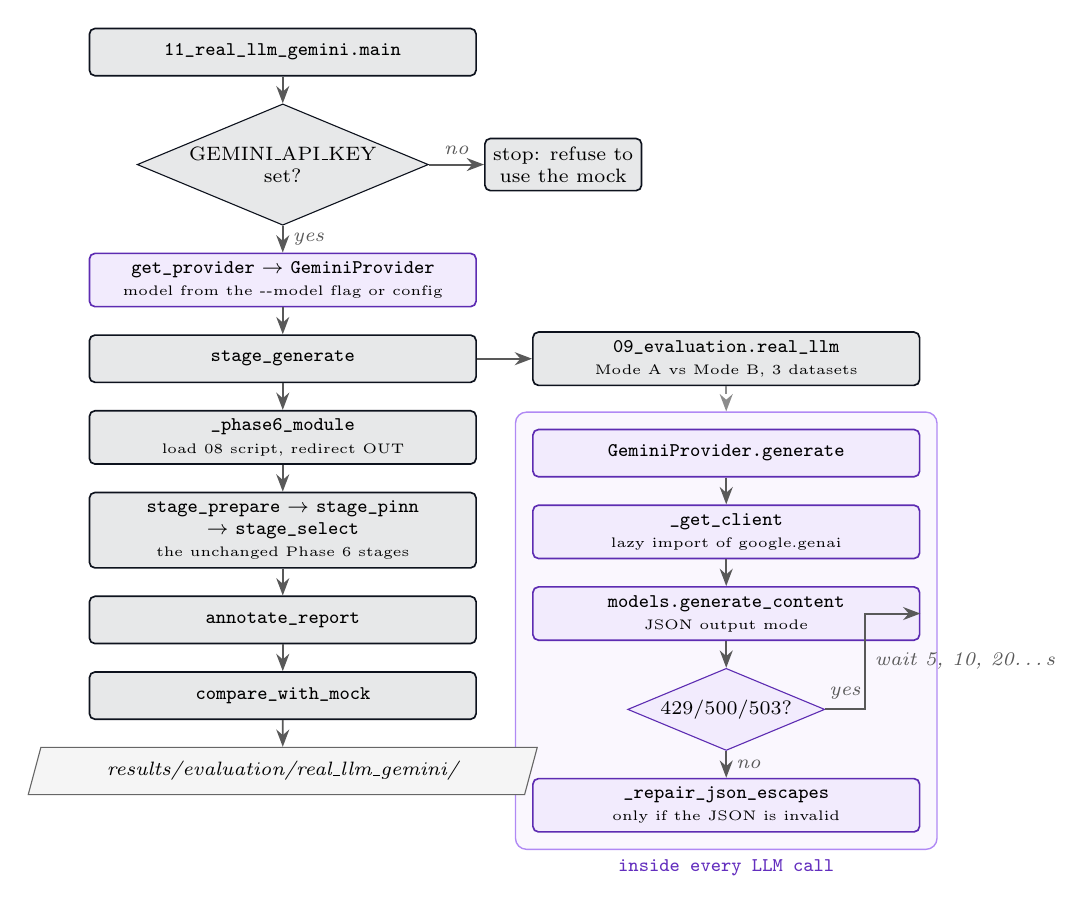
\begin{tikzpicture}[node distance=3.4mm and 7mm]
  \node[fnw=cExp] (main) {11_real_llm_gemini.main};
  \node[dec=cExp, below=of main] (key) {GEMINI_API_KEY\\set?};
  \node[fn=cExp, right=of key, font=\scriptsize] (stop) {stop: refuse to\\use the mock};
  \node[fnw=cLlm, below=of key] (gp) {get_provider $\to$ GeminiProvider\\{\normalfont\tiny model from the -{}-model flag or config}};
  \node[fnw=cExp, below=of gp] (sg) {stage_generate};
  \node[fnw=cExp, right=of sg] (rl) {09_evaluation.real_llm\\{\normalfont\tiny Mode A vs Mode B, 3 datasets}};
  \node[fnw=cExp, below=of sg] (p6) {_phase6_module\\{\normalfont\tiny load 08 script, redirect OUT}};
  \node[fnw=cExp, below=of p6] (st) {stage_prepare $\to$ stage_pinn\\$\to$ stage_select\\{\normalfont\tiny the unchanged Phase 6 stages}};
  \node[fnw=cExp, below=of st] (ar) {annotate_report};
  \node[fnw=cExp, below=of ar] (cm) {compare_with_mock};
  \node[io, below=of cm] (out) {results/evaluation/real\_llm\_gemini/};
  % provider internals
  \node[fnw=cLlm, right=of p6, yshift=-2mm] (gen) {GeminiProvider.generate};
  \node[fnw=cLlm, below=of gen] (cl) {_get_client\\{\normalfont\tiny lazy import of google.genai}};
  \node[fnw=cLlm, below=of cl] (gc) {models.generate_content\\{\normalfont\tiny JSON output mode}};
  \node[dec=cLlm, below=of gc] (err) {429/500/503?};
  \node[fnw=cLlm, below=of err] (rep) {_repair_json_escapes\\{\normalfont\tiny only if the JSON is invalid}};
  \begin{scope}[on background layer]
    \node[pkgbox=cLlm, fit=(gen)(cl)(gc)(err)(rep), label={[pkglabel=cLlm]below:inside every LLM call}] (box) {};
  \end{scope}
  \draw[flow] (main) -- (key); \draw[flow] (key) -- node[note, above]{no} (stop);
  \draw[flow] (key) -- node[note, right]{yes} (gp); \draw[flow] (gp) -- (sg); \draw[flow] (sg) -- (rl);
  \draw[flow] (sg) -- (p6); \draw[flow] (p6) -- (st); \draw[flow] (st) -- (ar); \draw[flow] (ar) -- (cm);
  \draw[flow] (cm) -- (out);
  \draw[flow] (gen) -- (cl); \draw[flow] (cl) -- (gc); \draw[flow] (gc) -- (err);
  \draw[flow] (err.east) -- node[note, above]{yes} ++(5mm,0) |- node[note, right, pos=0.25]{wait 5, 10, 20\ldots s} (gc.east);
  \draw[flow] (err) -- node[note, right]{no} (rep);
  \draw[dflow] (rl.south) -- (box.north -| rl.south);
\end{tikzpicture}

\pkglegend
\caption{The real-LLM run. Left: the runner reuses the existing stages. Right: what \fn{GeminiProvider.generate}
does on every call, including the two compatibility fixes added for Gemini.}
\label{fig:gemini}
\end{figure}

\subsection{Problems met, and the minimal fixes}

\begin{enumerate}
  \item \textbf{Overload.} The configured \fn{gemini-3.8-flash} (and \fn{gemini-3.5-flash}) repeatedly answered
        \emph{503: model is currently experiencing high demand}. The provider now retries 429/500/503 with
        increasing waits. When that was still not enough, the run used \fn{gemini-3.5-flash-lite}, passed with
        \fn{-{}-model} for that run only; the configuration was not changed.
  \item \textbf{Invalid JSON.} Gemini sometimes wrote \LaTeX{} such as \verb|\partial| inside JSON strings.
        That is an illegal escape, and the strict parser threw away the \emph{entire} response. The fix asks Gemini
        for its native JSON mode and, if the text still fails to parse, doubles stray backslashes.
\end{enumerate}
Neither fix touched the scientific pipeline. Many Gemini proposals were still (correctly) rejected by the project's
own validator, mostly because Gemini writes powers as \texttt{u\^{}3} where the compiler expects \texttt{u**3},
or uses $u_{xxxx}$, which is not in the derivative set.

\subsection{Results}

\textbf{Did evidence (RAG) change Gemini's hypotheses?} Yes, on all three test datasets.
\begin{center}
\small
\begin{tabular}{@{}p{2.8cm}p{5.6cm}p{5.6cm}@{}}
\toprule
\textbf{Dataset} & \textbf{Mode A (no evidence)} & \textbf{Mode B (with retrieved evidence)} \\ \midrule
diffusion & decay and logistic variants only; no plain diffusion & plain diffusion $u_t=D\,u_{xx}$ appears \\
reaction--diffusion & correct family $D\,u_{xx} + r\,u(1-u/K)$ & no valid hypothesis (one response failed schema) \\
advection--diffusion & correct family, velocity named $v$ & same family, renamed to the corpus's $c$ \\
\bottomrule
\end{tabular}
\end{center}

\textbf{Full Phase~6 pipeline with Gemini} (same data, splits and thresholds as the mock run):
\begin{center}
\small
\begin{tabular}{@{}>{\raggedright\arraybackslash}p{4.0cm}>{\raggedright\arraybackslash}p{5.4cm}>{\raggedright\arraybackslash}p{5.4cm}@{}}
\toprule
 & \textbf{Mock (Phase 6)} & \textbf{Gemini (gemini-3.5-flash-lite)} \\ \midrule
LLM candidates & $D\,u_{xx}$;\ $c\,u_x$ advection;\ reaction--diff.;\ adv.--diff. & $D\,u_{xx}$;\ $D\,u_{xx}-r\,u$;\ adv.--diff.;\ reaction--diff. \\
Graph templates added & K3 (pure reaction) & K1 (pure advection), K3 \\
Passed the gate & H1, H3, H4 & H1, H2, H3, H4 \\
Rejected & H2 (advection), K3 & K1 (advection), K3 \\
\textbf{Selected} & $u_t = D\,u_{xx}$ & $u_t = D\,u_{xx}$ \\
$\hat D$ (error) & 0.10002 (0.021\%) & 0.10001 (0.011\%) \\
Holdout RMSE & 0.01214 & 0.01218 \\
OOD RMSE, noisy obs. & 0.01144 & 0.01160 \\
OOD RMSE vs clean field (oracle) & 0.00181 & 0.00201 \\
Novel window $t\in(1,1.5]$ (oracle) & $2.5\times10^{-4}$ & $2.7\times10^{-4}$ \\
\bottomrule
\end{tabular}
\end{center}

Gemini's three more complex candidates all fit as well as diffusion, but their extra terms were judged inactive
($r\approx0.013$, $c\approx0.001$, $r\approx0.017$), each reduces to plain diffusion, and the same law won on
complexity and BIC. The real LLM proposed more physically plausible alternatives than the mock's canned pure
advection, and the pipeline reached the same, correct conclusion.

\begin{figure}[!htb]
\centering
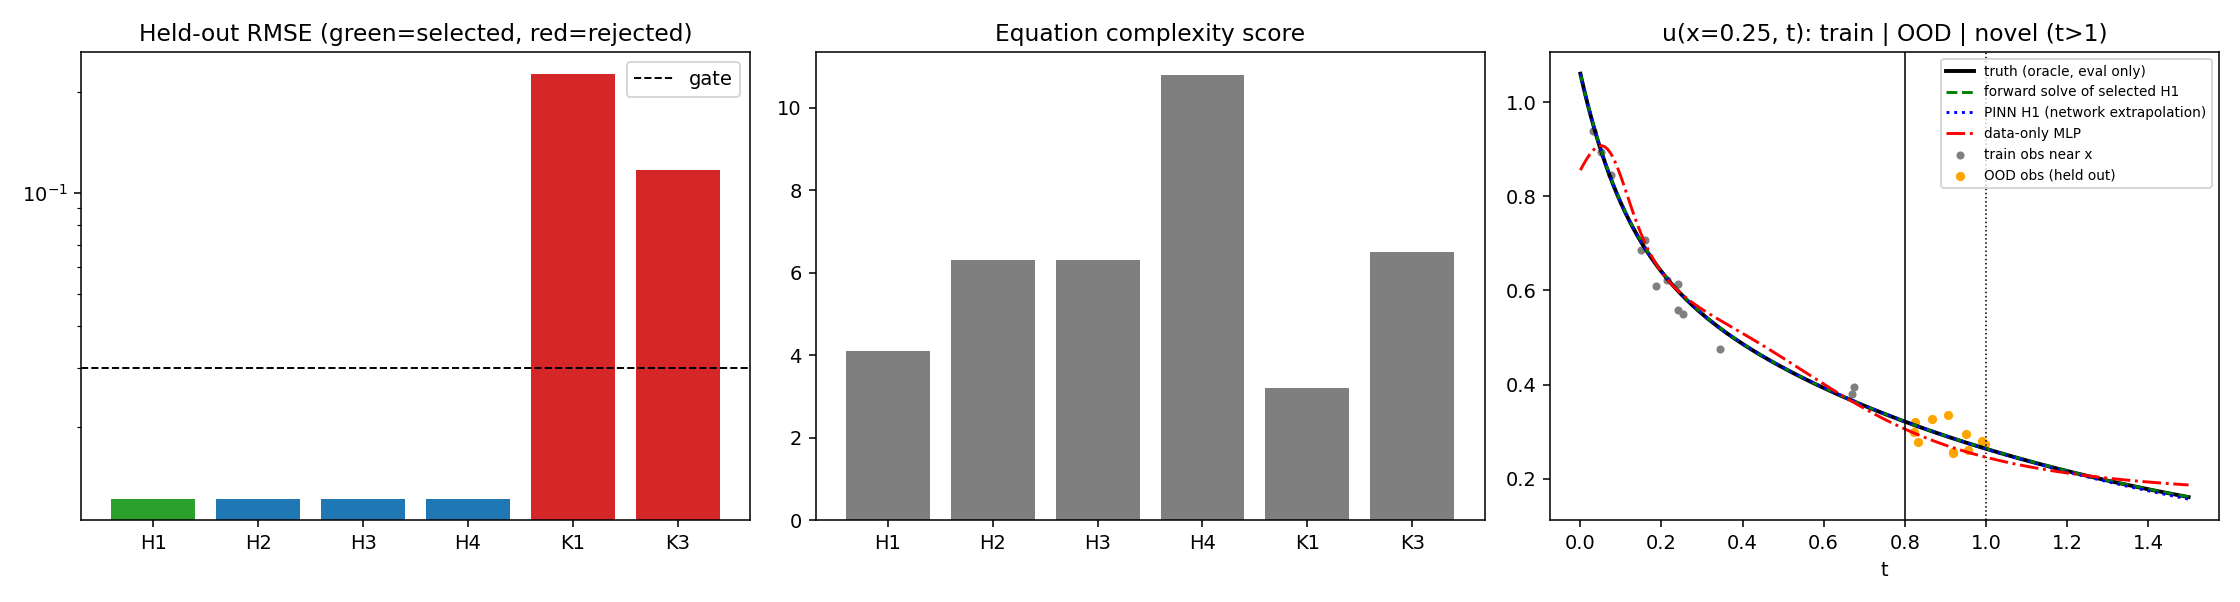
\includegraphics[width=\textwidth]{results/evaluation/real_llm_gemini/phase6/phase6_summary.png}
\caption{The Gemini run's Phase~6 summary (from \fn{results/evaluation/real_llm_gemini/phase6/}), in the same
layout as the mock run's figure.}
\end{figure}

\begin{caution}[: one sample]
LLM output is random from run to run. This is a single Gemini sample on one dataset; it shows the pipeline works
with a real LLM and that evidence changes the proposals, not that Gemini reliably discovers laws.
\end{caution}

% =====================================================================
\section{What is and is not demonstrated}\label{sec:limits}
% =====================================================================

The project's final report audits every claim. In short:
\begin{center}
\small
\begin{tabular}{@{}p{4.2cm}p{3.2cm}p{7.2cm}@{}}
\toprule
\textbf{Claim} & \textbf{Verdict} & \textbf{Why} \\ \midrule
PINN forward and inverse & demonstrated & $D$ and $c$ recovered within 0.4\% on two systems \\
Physics-constrained search & demonstrated & Phase~6 and the second system \\
OOD and novel prediction & demonstrated & both systems; physics-free network 6--40$\times$ worse \\
Adversarial robustness & demonstrated & 20/20 (3 by abstention) \\
LLM-driven discovery & partial (new) & one real Gemini run; same correct answer as the mock \\
RAG contribution & partial & recall only; top-1 retrieval 1/6 \\
Knowledge-graph contribution & partial & structured queries and provenance; no accuracy gain \\
Noisy-data robustness & partial & PINN path works at 5\% noise; SINDy fails \\
Uncertainty & partial & bootstrap only, not Bayesian; disagrees with the PINN on H3 \\
Equation uniqueness & not demonstrated & nested models fit equally; selection is a stated parsimony rule \\
Boundary/initial-condition inference & not demonstrated & supplied as known physics \\
Real-world data; a new law & not demonstrated & synthetic 1D data; known laws recovered \\
\bottomrule
\end{tabular}
\end{center}

\textbf{Main limitations.} Synthetic one-dimensional PDEs only; boundary and initial conditions are given, not
inferred; lexical (word-hashing) retrieval over a five-document corpus; hand-set thresholds (fixed in advance, but
not calibrated on independent data); the fast regression engine has no noise robustness; and uncertainty is a
bootstrap, not a posterior.

% =====================================================================
\section{Glossary}
% =====================================================================

\begin{description}[style=nextline, itemsep=1pt, font=\normalfont\bfseries]
  \item[Ablation] Removing one component at a time to measure how much it contributes.
  \item[Abstention] Declining to select any law when no candidate passes the gate. Safe, but not discovery.
  \item[Autograd] Automatic, exact differentiation of a neural network's output, used for $u_t, u_x, u_{xx}$ in PINNs.
  \item[BIC] Bayesian information criterion, $n\ln(\mathrm{MSE}) + k\ln n$: fit quality plus a penalty per parameter.
  \item[Canonical signature] An equation's structure with parameter names and signs normalised, for duplicate detection.
  \item[Collocation points] Random $(x,t)$ points where a PINN's equation residual is penalised; no data is needed there.
  \item[Complexity score] Terms + free parameters + derivative order + 2$\times$nonlinear terms + 0.1$\times$operations.
  \item[Embedding] A vector representing a piece of text, so similar texts get similar vectors.
  \item[Finite differences] Approximating derivatives from neighbouring grid values; amplifies noise.
  \item[Forward / inverse problem] Forward: parameters known, predict $u$. Inverse: estimate unknown parameters from data.
  \item[Gate] The pass/fail check on held-out error, physics residual, BC, IC and physical bounds.
  \item[Hypothesis] A candidate equation with its unknown parameters, in the \fn{Hypothesis} JSON schema.
  \item[Identifiability] Whether the data can distinguish two terms at all (the eigenfunction trap is a failure of it).
  \item[Knowledge graph] Typed entities and typed relationships, each with provenance.
  \item[Leakage] Any route by which the hidden answer could influence a decision.
  \item[Nested model] A model that contains another as a special case (reaction--diffusion with $r=0$ is diffusion).
  \item[OOD] Out-of-distribution: here, observations later than $t=0.8$ that no decision ever sees.
  \item[Oracle] The hidden truth, used only to report error after all decisions.
  \item[PINN] Physics-informed neural network: a network trained to fit data and obey an equation.
  \item[RAG] Retrieval-augmented generation: retrieve relevant documents and include them in the LLM prompt.
  \item[Residual] For an equation written as $\mathcal{R}=0$, the value of $\mathcal{R}$; zero when the equation holds.
  \item[SINDy / STLSQ] Sparse regression for equation discovery / its thresholded least-squares solver.
  \item[Term necessity] The share of $u_t$ a parameter's terms contribute; under 5\% means inactive.
\end{description}

\appendix
% generated by docs/gen_function_reference.py -- do not edit by hand
\section{Complete function reference}\label{app:functions}
Every function and class in the project (tests excluded), grouped by package and module, generated from the source code so that nothing is missed. Methods are listed as \texttt{Class.method}. In total: 284 entries in 70 modules.

\subsection*{\texttt{data/}}
\begin{longtable}{@{}>{\raggedright\arraybackslash}p{5.6cm}>{\raggedright\arraybackslash}p{10.6cm}@{}}
\multicolumn{2}{@{}l}{\small\bfseries\texttt{data/generate\_diffusion.py}}\\[1pt]
\quad\fn{load_config} & \small Read config.yaml into a dict. \\
\quad\fn{initial_condition} & \small The starting profile u(x,0): one sine (degenerate), two sines (default) or a Gaussian bump. \\
\quad\fn{solve_diffusion_fd} & \small Explicit finite-difference solver for u\_t = D u\_xx with zero boundary values; produces the ground truth. \\
\quad\fn{build_full_field} & \small Build the x and t grids from config and run the solver: the clean 800x61 field. \\
\quad\fn{flatten_field} & \small Turn the 2-D field into matching 1-D arrays (x, t, u), one row per grid point. \\
\quad\fn{make_sparse_and_noisy} & \small Draw the 10\% noise-free subsample and the 400 noisy observations (5\% noise). \\
\quad\fn{main} & \small Phase 1 entry point: generate and save full.npz, sparse.npz and noisy.npz. \\
\addlinespace[4pt]
\multicolumn{2}{@{}l}{\small\bfseries\texttt{data/problem\_description.py}}\\[1pt]
\quad\fn{build_problem_description} & \small Compute statistics of the noisy observations (amplitude change, edges, centroid, smoothness) and write them as plain text, never naming a mechanism. \\
\addlinespace[4pt]
\end{longtable}
\subsection*{\texttt{equation\_discovery/}}
\begin{longtable}{@{}>{\raggedright\arraybackslash}p{5.6cm}>{\raggedright\arraybackslash}p{10.6cm}@{}}
\multicolumn{2}{@{}l}{\small\bfseries\texttt{equation\_discovery/derivatives.py}}\\[1pt]
\quad\fn{reconstruct_grid} & \small Interpolate scattered (x, t, u) samples onto a regular grid (scipy griddata, nearest-neighbour at edges). \\
\quad\fn{smooth_grid} & \small Gaussian smoothing of a reconstructed grid to reduce noise before differentiation. \\
\quad\fn{finite_diff_derivatives} & \small Central finite differences on a grid: u\_t, u\_x, u\_xx, u\_xxx, with edge cropping. \\
\addlinespace[4pt]
\multicolumn{2}{@{}l}{\small\bfseries\texttt{equation\_discovery/discovery\_engine.py}}\\[1pt]
\quad\fn{_fields_from_grid} & \small Compute derivative fields on a grid and flatten them for regression. \\
\quad\fn{discover_from_grid} & \small Full discovery on gridded data: derivatives, library, sparse regression. \\
\quad\fn{discover_from_scatter} & \small Full discovery on scattered data: reconstruct, optionally smooth, then discover\_from\_grid. \\
\quad\fn{equation_to_string} & \small Format a discovery result as a readable equation string. \\
\quad\fn{evaluate_against_ground_truth} & \small Compare a discovered equation with the hidden truth (grading only, after discovery). \\
\quad\fn{evaluate_competing_hypotheses} & \small Fit each named single-term hypothesis separately and report R\^{}2 and coefficients. \\
\addlinespace[4pt]
\multicolumn{2}{@{}l}{\small\bfseries\texttt{equation\_discovery/library.py}}\\[1pt]
\quad\fn{term_label} & \small Human-readable label for a library term, e.g. ('u','u\_x') -> 'u*u\_x'. \\
\quad\fn{build_library} & \small Evaluate every candidate term at every sample: the matrix Theta. \\
\quad\fn{parse_term_specs} & \small Convert the config's term lists into term tuples. \\
\addlinespace[4pt]
\multicolumn{2}{@{}l}{\small\bfseries\texttt{equation\_discovery/sindy.py}}\\[1pt]
\quad\fn{stlsq} & \small Sequentially thresholded least squares: fit, zero small coefficients, refit, repeat (columns normalised). \\
\quad\fn{run_sindy} & \small Fit u\_t = Theta xi with STLSQ (pysindy if installed, else stlsq) and return a structured result. \\
\quad\fn{fit_restricted} & \small Ordinary least squares on a fixed set of terms (used for competing hypotheses). \\
\addlinespace[4pt]
\end{longtable}
\subsection*{\texttt{pinn/}}
\begin{longtable}{@{}>{\raggedright\arraybackslash}p{5.6cm}>{\raggedright\arraybackslash}p{10.6cm}@{}}
\multicolumn{2}{@{}l}{\small\bfseries\texttt{pinn/data\_utils.py}}\\[1pt]
\quad\fn{_to_tensor} & \small Convert a numpy array to a float32 column tensor. \\
\quad\fn{load_observational_data} & \small Load noisy.npz or sparse.npz, returning only x, t, u (the only data a PINN may train on). \\
\quad\fn{load_clean_reference} & \small Load the clean field for evaluation only, never for training. \\
\quad\fn{make_collocation_points} & \small Random (x, t) points where the physics residual is penalised. \\
\quad\fn{make_bc_points} & \small Random points on both boundaries with target u = 0. \\
\quad\fn{make_ic_points} & \small Random points at t = 0 with target u = initial condition. \\
\quad\fn{data_dict_to_tensors} & \small Convert an (x, t, u) dict into tensors. \\
\quad\fn{filter_by_time} & \small Keep only observations with t below a cutoff (train/OOD split). \\
\addlinespace[4pt]
\multicolumn{2}{@{}l}{\small\bfseries\texttt{pinn/derivatives.py}}\\[1pt]
\quad\fn{compute_derivatives} & \small Exact u, u\_t, u\_x, u\_xx (and u\_xxx) of the network output via torch.autograd. \\
\addlinespace[4pt]
\multicolumn{2}{@{}l}{\small\bfseries\texttt{pinn/forward.py}}\\[1pt]
\quad\fn{run_forward_pinn} & \small Train a PINN with physics parameters fixed (known D). \\
\addlinespace[4pt]
\multicolumn{2}{@{}l}{\small\bfseries\texttt{pinn/inverse.py}}\\[1pt]
\quad\fn{run_inverse_pinn} & \small Train a PINN with physics parameters trainable (estimate D). \\
\addlinespace[4pt]
\multicolumn{2}{@{}l}{\small\bfseries\texttt{pinn/losses.py}}\\[1pt]
\quad\fn{mse} & \small Mean squared error helper. \\
\quad\fn{data_loss} & \small Mismatch between network and observations. \\
\quad\fn{physics_loss} & \small Mean squared equation residual at collocation points. \\
\quad\fn{bc_loss} & \small Mismatch at the boundaries. \\
\quad\fn{ic_loss} & \small Mismatch with the initial condition. \\
\quad\fn{total_loss} & \small Weighted sum of the four losses. \\
\addlinespace[4pt]
\multicolumn{2}{@{}l}{\small\bfseries\texttt{pinn/network.py}}\\[1pt]
\quad\fn{PINN} & \small The one reusable network: (x, t) -> u through four tanh layers of 64 units. \\
\quad\fn{PINN._init_weights} & \small Xavier initialisation of the weights. \\
\quad\fn{PINN.forward} & \small Evaluate u at given (x, t). \\
\addlinespace[4pt]
\multicolumn{2}{@{}l}{\small\bfseries\texttt{pinn/residuals.py}}\\[1pt]
\quad\fn{diffusion_residual} & \small Residual u\_t - D u\_xx. \\
\quad\fn{advection_residual} & \small Residual u\_t - c u\_x. \\
\quad\fn{reaction_diffusion_residual} & \small Residual u\_t - D u\_xx + k u. \\
\quad\fn{make_params} & \small Wrap initial parameter values as tensors, trainable or fixed. \\
\addlinespace[4pt]
\multicolumn{2}{@{}l}{\small\bfseries\texttt{pinn/trainer.py}}\\[1pt]
\quad\fn{PINNTrainer} & \small Holds network, residual function, parameters and loss weights; runs training. \\
\quad\fn{PINNTrainer.trainable_parameters} & \small Network weights plus any trainable physics parameters. \\
\quad\fn{PINNTrainer.compute_losses} & \small One evaluation of all loss terms (derivatives, residual, data, BC, IC). \\
\quad\fn{PINNTrainer.train} & \small Adam steps then an L-BFGS polish, recording loss history. \\
\quad\fn{PINNTrainer._record} & \small Store one row of loss history and current parameter values. \\
\quad\fn{build_and_train} & \small Shared entry point: build network and parameters, train, return trainer and history. \\
\addlinespace[4pt]
\end{longtable}
\subsection*{\texttt{validation/}}
\begin{longtable}{@{}>{\raggedright\arraybackslash}p{5.6cm}>{\raggedright\arraybackslash}p{10.6cm}@{}}
\multicolumn{2}{@{}l}{\small\bfseries\texttt{validation/conservation.py}}\\[1pt]
\quad\fn{conservation_violation} & \small Global balance check: does the model's total amount change exactly as its own law says (dM/dt = integral of f)? \\
\addlinespace[4pt]
\multicolumn{2}{@{}l}{\small\bfseries\texttt{validation/forward\_solver.py}}\\[1pt]
\quad\fn{rhs_function} & \small Compile any candidate equation into a numerical right-hand side u\_t = f(u, u\_x, u\_xx). \\
\quad\fn{_effective_coefficients} & \small Estimate diffusion/advection/reaction strengths to choose a stable time step. \\
\quad\fn{solve_forward} & \small Solve a candidate law forward in time from an initial condition (Euler or RK4). \\
\addlinespace[4pt]
\multicolumn{2}{@{}l}{\small\bfseries\texttt{validation/model\_selection.py}}\\[1pt]
\quad\fn{parameter_contributions} & \small Term necessity: share of RMS(u\_t) contributed by each parameter's terms on the trained PINN. \\
\quad\fn{reduced_signature} & \small Signature of the equation with inactive terms removed (does it reduce to another candidate?). \\
\quad\fn{bic} & \small Bayesian information criterion n ln(MSE) + k ln n. \\
\quad\fn{select_model} & \small The selection rule: gate, fit-equivalence, optional reduction, complexity, BIC. \\
\addlinespace[4pt]
\multicolumn{2}{@{}l}{\small\bfseries\texttt{validation/ood.py}}\\[1pt]
\quad\fn{split_by_time} & \small Split points into t <= cutoff and t > cutoff. \\
\quad\fn{prediction_error} & \small RMSE and MAE of a model against reference values. \\
\addlinespace[4pt]
\multicolumn{2}{@{}l}{\small\bfseries\texttt{validation/physics\_validation.py}}\\[1pt]
\quad\fn{evaluate_physics_residual} & \small Mean squared residual of a trained PINN on a fresh grid (not the training points). \\
\addlinespace[4pt]
\multicolumn{2}{@{}l}{\small\bfseries\texttt{validation/scorer.py}}\\[1pt]
\quad\fn{build_validation_result} & \small Turn measured losses into supported/rejected using fixed thresholds (Phase 3). \\
\addlinespace[4pt]
\multicolumn{2}{@{}l}{\small\bfseries\texttt{validation/stability.py}}\\[1pt]
\quad\fn{candidate_monomials} & \small The distinct field terms on a candidate's right-hand side (e.g. u\_xx, u, u\^{}2). \\
\quad\fn{bootstrap_stability} & \small Refit those terms by least squares on 20 random 80\% subsets; report mean, spread, sign stability. \\
\addlinespace[4pt]
\end{longtable}
\subsection*{\texttt{llm/}}
\begin{longtable}{@{}>{\raggedright\arraybackslash}p{5.6cm}>{\raggedright\arraybackslash}p{10.6cm}@{}}
\multicolumn{2}{@{}l}{\small\bfseries\texttt{llm/\_\_init\_\_.py}}\\[1pt]
\quad\fn{get_provider} & \small Choose the LLM provider from config and environment (Gemini if a key is set, else the mock). \\
\addlinespace[4pt]
\multicolumn{2}{@{}l}{\small\bfseries\texttt{llm/base.py}}\\[1pt]
\quad\fn{LLMProvider} & \small Abstract interface every LLM provider implements. \\
\quad\fn{LLMProvider.generate} & \small Return the raw text completion for a prompt. \\
\quad\fn{LLMProvider.name} & \small The provider's class name, recorded in results. \\
\addlinespace[4pt]
\multicolumn{2}{@{}l}{\small\bfseries\texttt{llm/gemini\_provider.py}}\\[1pt]
\quad\fn{_repair_json_escapes} & \small If the response is not valid JSON, double stray backslashes (LaTeX like \textbackslash{}partial). \\
\quad\fn{GeminiProvider} & \small Real provider for Google Gemini; the key comes only from GEMINI\_API\_KEY. \\
\quad\fn{GeminiProvider._get_client} & \small Lazily import google-genai and create the client; clear error if no key. \\
\quad\fn{GeminiProvider.generate} & \small Call Gemini in JSON mode, retrying overload errors (429/500/503) with back-off. \\
\addlinespace[4pt]
\multicolumn{2}{@{}l}{\small\bfseries\texttt{llm/mock\_provider.py}}\\[1pt]
\quad\fn{MockLLMProvider} & \small Deterministic offline provider returning a canned set of four hypotheses. \\
\quad\fn{MockLLMProvider.generate} & \small Return the same canned JSON every time, whatever the prompt. \\
\addlinespace[4pt]
\multicolumn{2}{@{}l}{\small\bfseries\texttt{llm/openai\_provider.py}}\\[1pt]
\quad\fn{OpenAIProvider} & \small Legacy OpenAI provider (no longer selectable by get\_provider). \\
\quad\fn{OpenAIProvider._get_client} & \small Lazily create the OpenAI client. \\
\quad\fn{OpenAIProvider.generate} & \small Call OpenAI chat completions. \\
\addlinespace[4pt]
\multicolumn{2}{@{}l}{\small\bfseries\texttt{llm/prompts.py}}\\[1pt]
\quad\fn{build_hypothesis_prompt_with_context} & \small Mode B prompt: observations plus retrieved evidence, mechanisms, equations and parameters. \\
\quad\fn{build_hypothesis_prompt} & \small Mode A prompt: observations only, with the JSON schema the answer must follow. \\
\addlinespace[4pt]
\multicolumn{2}{@{}l}{\small\bfseries\texttt{llm/schemas.py}}\\[1pt]
\quad\fn{ParameterSpec} & \small One parameter: name, trainable flag, initial value, units, optional bounds. \\
\quad\fn{Hypothesis} & \small The structured hypothesis every LLM answer must fit (pydantic model). \\
\quad\fn{Hypothesis._confidence_in_range} & \small Validator: confidence must lie in [0, 1]. \\
\quad\fn{Hypothesis._equation_has_equals} & \small Validator: the equation must contain '='. \\
\quad\fn{HypothesisSet} & \small A validated collection of hypotheses for one problem. \\
\addlinespace[4pt]
\end{longtable}
\subsection*{\texttt{hypotheses/}}
\begin{longtable}{@{}>{\raggedright\arraybackslash}p{5.6cm}>{\raggedright\arraybackslash}p{10.6cm}@{}}
\multicolumn{2}{@{}l}{\small\bfseries\texttt{hypotheses/adapter.py}}\\[1pt]
\quad\fn{hypothesis_to_pinn_config} & \small Compile a hypothesis into exactly what build\_and\_train needs (residual function, parameters). \\
\addlinespace[4pt]
\multicolumn{2}{@{}l}{\small\bfseries\texttt{hypotheses/complexity.py}}\\[1pt]
\quad\fn{equation_complexity} & \small Complexity score: terms + free parameters + derivative order + 2 x nonlinear + 0.1 x operations. \\
\addlinespace[4pt]
\multicolumn{2}{@{}l}{\small\bfseries\texttt{hypotheses/constraints.py}}\\[1pt]
\quad\fn{resolve_bounds} & \small Combine a hypothesis's declared bounds with the config fallbacks (D > 0, K > 0). \\
\quad\fn{precheck_physics} & \small Before training: reject non-evolution equations; warn on over-determined or uncoupled boundary setups. \\
\quad\fn{check_fitted_bounds} & \small After training: flag fitted parameters that violate physical bounds. \\
\addlinespace[4pt]
\multicolumn{2}{@{}l}{\small\bfseries\texttt{hypotheses/equation\_compiler.py}}\\[1pt]
\quad\fn{EquationParseError} & \small Raised when an equation string cannot be parsed. \\
\quad\fn{parse_equation} & \small Parse 'lhs = rhs' with SymPy into a residual; detect fields and parameters used. \\
\quad\fn{compile_residual} & \small Turn the residual into a torch function residual\_fn(derivs, params) for the trainer. \\
\quad\fn{equation_str_to_sympy_str} & \small Normalised human-readable form of an equation. \\
\addlinespace[4pt]
\multicolumn{2}{@{}l}{\small\bfseries\texttt{hypotheses/pipeline.py}}\\[1pt]
\quad\fn{_extract_json_array} & \small Strip markdown code fences and parse the LLM's JSON array. \\
\quad\fn{generate_hypotheses} & \small Prompt, call the provider, parse, schema-check, validate, deduplicate and rank. \\
\addlinespace[4pt]
\multicolumn{2}{@{}l}{\small\bfseries\texttt{hypotheses/ranking.py}}\\[1pt]
\quad\fn{_completeness_score} & \small Fraction of descriptive fields the LLM filled in. \\
\quad\fn{_simplicity_score} & \small 1 / (1 + number of parameters). \\
\quad\fn{rank_hypotheses} & \small Composite score that sets investigation order only, never the verdict. \\
\addlinespace[4pt]
\multicolumn{2}{@{}l}{\small\bfseries\texttt{hypotheses/search.py}}\\[1pt]
\quad\fn{kg_template_candidates} & \small Turn equations documented in the knowledge graph into candidate hypotheses. \\
\quad\fn{build_candidate_pool} & \small Merge LLM and graph candidates and remove structural duplicates. \\
\quad\fn{structural_and_physics_filter} & \small Run deterministic validation and physics pre-checks; keep the survivors. \\
\quad\fn{make_splits} & \small Train / random holdout / OOD (t > cutoff) splits of the observations. \\
\quad\fn{_rmse} & \small RMSE of a network on a split. \\
\quad\fn{validate_candidate} & \small Inverse PINN on the training split, then gate checks, bounds, term necessity, complexity, BIC. \\
\quad\fn{load_candidate_model} & \small Reload a saved candidate network. \\
\quad\fn{train_data_only_mlp} & \small Baseline: the same network trained on data only, without physics. \\
\quad\fn{save_json} & \small Write a result dict to JSON, creating folders as needed. \\
\addlinespace[4pt]
\multicolumn{2}{@{}l}{\small\bfseries\texttt{hypotheses/validation.py}}\\[1pt]
\quad\fn{validate_hypothesis} & \small Deterministic checks: syntax, variables, parameters, derivatives, units. \\
\quad\fn{canonical_signature} & \small Parameter- and sign-invariant structure of an equation, for duplicate detection. \\
\quad\fn{deduplicate} & \small Remove hypotheses with identical canonical signatures. \\
\addlinespace[4pt]
\end{longtable}
\subsection*{\texttt{rag/}}
\begin{longtable}{@{}>{\raggedright\arraybackslash}p{5.6cm}>{\raggedright\arraybackslash}p{10.6cm}@{}}
\multicolumn{2}{@{}l}{\small\bfseries\texttt{rag/chunker.py}}\\[1pt]
\quad\fn{chunk_document} & \small Split a document into chunks at its section headers. \\
\addlinespace[4pt]
\multicolumn{2}{@{}l}{\small\bfseries\texttt{rag/context.py}}\\[1pt]
\quad\fn{ScientificContext} & \small The unified evidence object: retrieved evidence, mechanisms, equations, parameters, sources. \\
\quad\fn{build_scientific_context} & \small Retrieve evidence for the description, then query the graph for every mechanism it mentions. \\
\addlinespace[4pt]
\multicolumn{2}{@{}l}{\small\bfseries\texttt{rag/corpus\_loader.py}}\\[1pt]
\quad\fn{_parse_frontmatter} & \small Split a Markdown file into its metadata header and body. \\
\quad\fn{load_document} & \small Load one corpus file as a Document. \\
\quad\fn{load_corpus} & \small Load every .md file in rag/corpus/. \\
\addlinespace[4pt]
\multicolumn{2}{@{}l}{\small\bfseries\texttt{rag/documents.py}}\\[1pt]
\quad\fn{DocumentMetadata} & \small A document's id, title, source, domain and declared mechanism, equations and parameters. \\
\quad\fn{Document} & \small Metadata plus text. \\
\quad\fn{Chunk} & \small A piece of a document with its section and id. \\
\addlinespace[4pt]
\multicolumn{2}{@{}l}{\small\bfseries\texttt{rag/embeddings.py}}\\[1pt]
\quad\fn{EmbeddingProvider} & \small Interface for turning text into vectors. \\
\quad\fn{EmbeddingProvider.embed} & \small Embed one text. \\
\quad\fn{EmbeddingProvider.embed_many} & \small Embed many texts. \\
\quad\fn{EmbeddingProvider.name} & \small Provider name. \\
\quad\fn{LocalEmbeddingProvider} & \small Deterministic offline embedding: words hashed into 256 slots, normalised. \\
\quad\fn{LocalEmbeddingProvider._token_index} & \small Hash a word to a slot (MD5 modulo 256). \\
\quad\fn{LocalEmbeddingProvider.embed} & \small Count words per slot and normalise to unit length. \\
\quad\fn{APIEmbeddingProvider} & \small Optional real embedding API provider (unused by default). \\
\quad\fn{APIEmbeddingProvider._get_client} & \small Lazily create its API client. \\
\quad\fn{APIEmbeddingProvider.embed} & \small Embed via the API. \\
\addlinespace[4pt]
\multicolumn{2}{@{}l}{\small\bfseries\texttt{rag/evidence.py}}\\[1pt]
\quad\fn{RetrievalResult} & \small One retrieved chunk with its similarity score. \\
\quad\fn{Evidence} & \small A retrieved claim with provenance; its confidence is retrieval confidence only. \\
\quad\fn{evidence_from_retrieval} & \small Convert a retrieval result into an Evidence object. \\
\addlinespace[4pt]
\multicolumn{2}{@{}l}{\small\bfseries\texttt{rag/metadata.py}}\\[1pt]
\quad\fn{matches_filters} & \small Check a chunk's metadata against filter values. \\
\addlinespace[4pt]
\multicolumn{2}{@{}l}{\small\bfseries\texttt{rag/pipeline.py}}\\[1pt]
\quad\fn{RAGPipeline} & \small Ties chunker, embedder and vector store together. \\
\quad\fn{RAGPipeline.ingest} & \small Chunk, embed and store every document. \\
\quad\fn{RAGPipeline.get_retriever} & \small Return a Retriever over the stored chunks. \\
\addlinespace[4pt]
\multicolumn{2}{@{}l}{\small\bfseries\texttt{rag/retriever.py}}\\[1pt]
\quad\fn{Retriever} & \small Search interface over the vector store. \\
\quad\fn{Retriever.retrieve} & \small Embed the query, take the most similar chunks, apply filters, return Evidence. \\
\addlinespace[4pt]
\multicolumn{2}{@{}l}{\small\bfseries\texttt{rag/vector\_store.py}}\\[1pt]
\quad\fn{VectorStore} & \small Interface: add, search, get. \\
\quad\fn{VectorStore.add} & \small Store a vector with its payload. \\
\quad\fn{VectorStore.search} & \small Return the top-k most similar vectors. \\
\quad\fn{VectorStore.get} & \small Fetch one stored item. \\
\quad\fn{InMemoryVectorStore} & \small Brute-force cosine-similarity store in memory. \\
\quad\fn{InMemoryVectorStore.add} & \small Store a vector with its payload. \\
\quad\fn{InMemoryVectorStore.search} & \small Cosine similarity against every stored vector; return the top-k. \\
\quad\fn{InMemoryVectorStore.get} & \small Fetch one stored item. \\
\quad\fn{InMemoryVectorStore.all_ids} & \small List stored ids. \\
\quad\fn{PersistentVectorStore} & \small The in-memory store plus JSON save/load. \\
\quad\fn{PersistentVectorStore.save} & \small Write the store to JSON. \\
\quad\fn{PersistentVectorStore.load} & \small Read the store from JSON. \\
\addlinespace[4pt]
\end{longtable}
\subsection*{\texttt{knowledge\_graph/}}
\begin{longtable}{@{}>{\raggedright\arraybackslash}p{5.6cm}>{\raggedright\arraybackslash}p{10.6cm}@{}}
\multicolumn{2}{@{}l}{\small\bfseries\texttt{knowledge\_graph/builder.py}}\\[1pt]
\quad\fn{_slug} & \small Make a stable id fragment from a name. \\
\quad\fn{_find_chunk_id} & \small Find the chunk that states a fact (provenance). \\
\quad\fn{build_graph_from_documents} & \small Create Document, Mechanism, Equation, Variable and Parameter entities and sourced relationships. \\
\addlinespace[4pt]
\multicolumn{2}{@{}l}{\small\bfseries\texttt{knowledge\_graph/graph.py}}\\[1pt]
\quad\fn{_relationship_id} & \small Stable hash of (subject, predicate, object), so repeated facts merge. \\
\quad\fn{KnowledgeGraph} & \small The graph container (backed by networkx). \\
\quad\fn{KnowledgeGraph.add_entity} & \small Add an entity, merging if its id exists. \\
\quad\fn{KnowledgeGraph.get_entity} & \small Look up an entity by id. \\
\quad\fn{KnowledgeGraph.entities_by_type} & \small All entities of one type. \\
\quad\fn{KnowledgeGraph.add_relationship} & \small Add a typed, sourced edge, merging sources for duplicates. \\
\quad\fn{KnowledgeGraph.neighbors} & \small Entities connected to a given entity. \\
\quad\fn{KnowledgeGraph.relationships_for} & \small Edges touching a given entity. \\
\quad\fn{KnowledgeGraph.summary} & \small Counts of entities and relationships by type. \\
\addlinespace[4pt]
\multicolumn{2}{@{}l}{\small\bfseries\texttt{knowledge\_graph/query.py}}\\[1pt]
\quad\fn{find_entity_by_name} & \small Find an entity by its name. \\
\quad\fn{equations_for_mechanism} & \small Documented equations that govern a mechanism. \\
\quad\fn{variables_for_mechanism} & \small Variables in those equations. \\
\quad\fn{parameters_for_mechanism} & \small Parameters in those equations. \\
\quad\fn{mechanisms_for_observation} & \small Mechanisms linked to an observation entity (schema-ready). \\
\quad\fn{documents_supporting} & \small Documents that support an entity. \\
\quad\fn{sources_for_relationship} & \small Provenance of an edge. \\
\quad\fn{evidence_connecting} & \small Relationships and shared equations linking two variables. \\
\addlinespace[4pt]
\multicolumn{2}{@{}l}{\small\bfseries\texttt{knowledge\_graph/schema.py}}\\[1pt]
\quad\fn{EntityType} & \small Allowed entity types (Document, Mechanism, Variable, Parameter, Equation, Observation). \\
\quad\fn{RelationType} & \small Allowed relationship types: GOVERNS, HAS\_VARIABLE, HAS\_PARAMETER, SUPPORTED\_BY, CAUSES, DEPENDS\_ON, and others. \\
\quad\fn{Entity} & \small A node: id, type, name, metadata. \\
\quad\fn{SourceRef} & \small Where a fact came from: document and chunk. \\
\quad\fn{Relationship} & \small A typed edge with its sources. \\
\addlinespace[4pt]
\multicolumn{2}{@{}l}{\small\bfseries\texttt{knowledge\_graph/serialization.py}}\\[1pt]
\quad\fn{graph_to_dict} & \small Convert the graph to a JSON-able dict. \\
\quad\fn{graph_from_dict} & \small Rebuild a graph from that dict. \\
\quad\fn{save_graph} & \small Write the graph to a JSON file. \\
\quad\fn{load_graph} & \small Read a graph from a JSON file. \\
\addlinespace[4pt]
\end{longtable}
\subsection*{\texttt{evaluation/}}
\begin{longtable}{@{}>{\raggedright\arraybackslash}p{5.6cm}>{\raggedright\arraybackslash}p{10.6cm}@{}}
\multicolumn{2}{@{}l}{\small\bfseries\texttt{evaluation/ablation.py}}\\[1pt]
\quad\fn{_discovery_only} & \small The SINDy-alone arm: discover, then match the result to a documented mechanism. \\
\quad\fn{run_ablation} & \small Run all seven arms on the 12 datasets. \\
\quad\fn{_median} & \small Median helper. \\
\quad\fn{summarize_ablation} & \small Per-arm totals: correct model, wrong candidates rejected, parameter and OOD accuracy. \\
\addlinespace[4pt]
\multicolumn{2}{@{}l}{\small\bfseries\texttt{evaluation/adversarial.py}}\\[1pt]
\quad\fn{_CannedProvider} & \small Test LLM that returns a fixed (possibly malicious) response. \\
\quad\fn{_CannedProvider.generate} & \small Return the canned response. \\
\quad\fn{_H} & \small Shorthand to build a test Hypothesis. \\
\quad\fn{_case} & \small Record one adversarial case result. \\
\quad\fn{find_leaks} & \small Search corpus text for any hidden benchmark value. \\
\quad\fn{run_adversarial} & \small Run the 20 attack cases. \\
\addlinespace[4pt]
\multicolumn{2}{@{}l}{\small\bfseries\texttt{evaluation/benchmark.py}}\\[1pt]
\quad\fn{_item} & \small Record one question result. \\
\quad\fn{_hyp} & \small Build a Hypothesis from an equation string, inferring parameter names. \\
\quad\fn{run_single_questions} & \small The 50 single questions over the 12 datasets and the graph. \\
\quad\fn{run_multihop} & \small The 25 multi-hop chains. \\
\addlinespace[4pt]
\multicolumn{2}{@{}l}{\small\bfseries\texttt{evaluation/datasets.py}}\\[1pt]
\quad\fn{Dataset} & \small One benchmark system: family, truth, grids, field, initial condition, exact solution. \\
\quad\fn{_diffusion} & \small Exact two-mode diffusion dataset. \\
\quad\fn{_gauss} & \small Exact moving, spreading Gaussian; used for advection (D = 0) and advection-diffusion. \\
\quad\fn{_advection} & \small Pure advection dataset. \\
\quad\fn{_adv_diff} & \small Advection-diffusion dataset. \\
\quad\fn{_reaction_diffusion} & \small Reaction-diffusion dataset solved numerically with RK4. \\
\quad\fn{benchmark_datasets} & \small The 12 datasets (4 families x 3 settings), cached to .npz. \\
\quad\fn{_build_all} & \small Construct all 12 datasets. \\
\quad\fn{_rd_shell} & \small Reaction-diffusion dataset without its (expensive) field, for quick metadata. \\
\quad\fn{add_noise} & \small Add Gaussian noise to a dataset's field. \\
\addlinespace[4pt]
\multicolumn{2}{@{}l}{\small\bfseries\texttt{evaluation/describe.py}}\\[1pt]
\quad\fn{_centroid} & \small Amplitude-weighted centre of a profile. \\
\quad\fn{_spread} & \small Width of a profile. \\
\quad\fn{_n_peaks} & \small Number of peaks in a profile. \\
\quad\fn{observation_stats} & \small Amplitude change, drift, spread and peaks between early and late times. \\
\quad\fn{describe_observations} & \small Fixed-template text description from those statistics (never names a mechanism). \\
\addlinespace[4pt]
\multicolumn{2}{@{}l}{\small\bfseries\texttt{evaluation/engine.py}}\\[1pt]
\quad\fn{Resources} & \small Corpus, RAG index and graph, built once and shared. \\
\quad\fn{build_pool} & \small Description -> RAG/graph context -> candidate pool (evidence equations, graph templates, mock LLM). \\
\quad\fn{_grid_param_contributions} & \small Term necessity computed on grid derivatives instead of a PINN. \\
\quad\fn{_reduced_term_set} & \small Term set of an equation with its inactive terms removed. \\
\quad\fn{validate_and_select} & \small Fast pipeline: least-squares fit per candidate, gate, selection. \\
\quad\fn{predict_ood} & \small Solve the selected law forward beyond the data window. \\
\quad\fn{family_of} & \small Map a hypothesis's term set to its mechanism family. \\
\quad\fn{truth_field} & \small Ground-truth field at given times (evaluation only). \\
\quad\fn{score_run} & \small Score one run: correct family, parameter error, OOD error. \\
\quad\fn{family_of_row} & \small Mechanism family from a stored result row. \\
\addlinespace[4pt]
\multicolumn{2}{@{}l}{\small\bfseries\texttt{evaluation/identify.py}}\\[1pt]
\quad\fn{_syms} & \small SymPy symbols for the fields. \\
\quad\fn{term_set} & \small The set of field terms in a hypothesis. \\
\quad\fn{_label_to_expr} & \small Convert a library label like 'u*u\_x' to a SymPy expression. \\
\quad\fn{discovered_coefficients} & \small Non-zero SINDy coefficients as \{term: value\}. \\
\quad\fn{match_mechanism} & \small Find the documented template with exactly the discovered term set. \\
\quad\fn{recover_parameters} & \small Solve for a template's parameters from discovered coefficients. \\
\quad\fn{grid_fields} & \small Finite-difference fields of a gridded dataset, flattened. \\
\quad\fn{fit_candidate_on_grid} & \small Least-squares fit of u\_t on a candidate's own terms; train and holdout error. \\
\quad\fn{library_collinearity} & \small Identifiability check: maximum correlation between library columns. \\
\addlinespace[4pt]
\multicolumn{2}{@{}l}{\small\bfseries\texttt{evaluation/leakage.py}}\\[1pt]
\quad\fn{ground_truth_references} & \small List ground-truth identifiers mentioned in a function's source code. \\
\quad\fn{decision_functions} & \small The six functions that make decisions (pool, validation, splits, selection). \\
\quad\fn{leakage_audit} & \small Static audit of those functions plus a corpus scan for hidden values. \\
\addlinespace[4pt]
\end{longtable}
\subsection*{\texttt{experiments/}}
\begin{longtable}{@{}>{\raggedright\arraybackslash}p{5.6cm}>{\raggedright\arraybackslash}p{10.6cm}@{}}
\multicolumn{2}{@{}l}{\small\bfseries\texttt{experiments/02\_equation\_discovery.py}}\\[1pt]
\quad\fn{load_config} & \small Read config.yaml. \\
\quad\fn{run_case} & \small Run discovery on one dataset variant and evaluate it. \\
\quad\fn{main} & \small Phase 2: clean, sparse, noisy (raw and smoothed); save report, table and plot. \\
\addlinespace[4pt]
\multicolumn{2}{@{}l}{\small\bfseries\texttt{experiments/03\_forward\_pinn.py}}\\[1pt]
\quad\fn{load_config} & \small Read config.yaml. \\
\quad\fn{main} & \small Phase 3 forward PINN with D = 0.1 fixed. \\
\addlinespace[4pt]
\multicolumn{2}{@{}l}{\small\bfseries\texttt{experiments/04\_inverse\_pinn.py}}\\[1pt]
\quad\fn{load_config} & \small Read config.yaml. \\
\quad\fn{main} & \small Phase 3 inverse PINN estimating D from 0.2. \\
\addlinespace[4pt]
\multicolumn{2}{@{}l}{\small\bfseries\texttt{experiments/05\_hypothesis\_validation.py}}\\[1pt]
\quad\fn{load_config} & \small Read config.yaml. \\
\quad\fn{run_hypothesis} & \small Train one hypothesis's PINN and score it. \\
\quad\fn{main} & \small Phase 3: diffusion vs advection with a time-based OOD split. \\
\addlinespace[4pt]
\multicolumn{2}{@{}l}{\small\bfseries\texttt{experiments/06\_hypothesis\_generation.py}}\\[1pt]
\quad\fn{load_config} & \small Read config.yaml. \\
\quad\fn{main} & \small Phase 4: generate, validate and rank hypotheses; optionally run PINNs. \\
\addlinespace[4pt]
\multicolumn{2}{@{}l}{\small\bfseries\texttt{experiments/07\_scientific\_rag\_kg.py}}\\[1pt]
\quad\fn{load_config} & \small Read config.yaml. \\
\quad\fn{hyp_to_dict} & \small Serialise a hypothesis. \\
\quad\fn{summarize_generation} & \small Counts for a generation run (candidates, valid, duplicates, evidence-supported). \\
\quad\fn{main} & \small Phase 5: corpus, RAG, graph, context, leakage check, Mode A vs Mode B. \\
\addlinespace[4pt]
\multicolumn{2}{@{}l}{\small\bfseries\texttt{experiments/08\_physics\_constrained\_search.py}}\\[1pt]
\quad\fn{load_config} & \small Read config.yaml. \\
\quad\fn{stage_prepare} & \small Phase 6 stage 1: context, generation, pool, filters. \\
\quad\fn{_load_survivors} & \small Reload the filtered candidates. \\
\quad\fn{_splits} & \small Build train/holdout/OOD splits from noisy.npz. \\
\quad\fn{_setup} & \small Domain and initial-condition settings for the PINN. \\
\quad\fn{stage_pinn} & \small Phase 6 stage 2: inverse PINN per survivor, cached. \\
\quad\fn{oracle_evaluation} & \small Benchmark-only error against the hidden truth, after selection. \\
\quad\fn{stage_select} & \small Phase 6 stage 3: stability, selection, baselines, OOD, novel prediction, report. \\
\quad\fn{_plots} & \small Draw the Phase 6 summary figure. \\
\quad\fn{_report} & \small Write phase6\_report.md. \\
\quad\fn{main} & \small Run the chosen stages. \\
\addlinespace[4pt]
\multicolumn{2}{@{}l}{\small\bfseries\texttt{experiments/09\_evaluation.py}}\\[1pt]
\quad\fn{save} & \small Write one Phase 7 result file. \\
\quad\fn{real_llm} & \small Mode A vs Mode B with a real LLM on 3 datasets (only with -{}-real-llm and a key). \\
\quad\fn{acc} & \small Format an accuracy fraction. \\
\quad\fn{report} & \small Write phase7\_report.md. \\
\quad\fn{main} & \small Phase 7: questions, multi-hop, adversarial, ablation, leakage, determinism check, report. \\
\addlinespace[4pt]
\multicolumn{2}{@{}l}{\small\bfseries\texttt{experiments/10\_generalization.py}}\\[1pt]
\quad\fn{_truth_dataset} & \small The hidden advection-diffusion system (c = 0.4, D = 0.02). \\
\quad\fn{observations} & \small 400 noisy samples, the only data the pipeline sees. \\
\quad\fn{_recon} & \small Grid reconstruction for SINDy and the description. \\
\quad\fn{_setup} & \small Domain settings for the PINN. \\
\quad\fn{stage_prepare} & \small SINDy baseline, pool and filters for the new system. \\
\quad\fn{_survivors} & \small Reload filtered candidates. \\
\quad\fn{_splits} & \small Train/holdout/OOD splits. \\
\quad\fn{stage_pinn} & \small Inverse PINN per candidate. \\
\quad\fn{stage_select} & \small Selection under both rules, OOD, oracle evaluation. \\
\quad\fn{main} & \small Run the chosen stages. \\
\addlinespace[4pt]
\multicolumn{2}{@{}l}{\small\bfseries\texttt{experiments/11\_real\_llm\_gemini.py}}\\[1pt]
\quad\fn{_load_script} & \small Import an experiment script by file path. \\
\quad\fn{_phase6_module} & \small Load the Phase 6 script and redirect its outputs to the Gemini folder. \\
\quad\fn{stage_generate} & \small Run 09's real\_llm Mode A vs Mode B with Gemini. \\
\quad\fn{annotate_report} & \small Mark the reused Phase 6 report as a real-LLM run. \\
\quad\fn{compare_with_mock} & \small Side-by-side summary of the mock and Gemini Phase 6 runs. \\
\quad\fn{main} & \small Check the key, force the Gemini provider, run the chosen stages. \\
\addlinespace[4pt]
\multicolumn{2}{@{}l}{\small\bfseries\texttt{experiments/12\_conservation.py}}\\[1pt]
\quad\fn{_windows} & \small Conservation violation in the train, OOD and beyond-data windows. \\
\quad\fn{evaluate_run} & \small Conservation check for every saved candidate of one Phase 6 run (no retraining). \\
\quad\fn{main} & \small Check the mock and Gemini runs plus the physics-free baseline; write results/evaluation/conservation/. \\
\addlinespace[4pt]
\end{longtable}

% =====================================================================
\section{Running the project yourself}\label{app:running}
% =====================================================================

All commands run from the project root (\fn{scientific-discovery-engine/}).

\subsection*{Install and test}
\begin{verbatim}
python -m pip install -r requirements.txt
python -m pytest tests -q            # 94 tests, no API key or network needed
\end{verbatim}

\subsection*{Reproduce each phase}
\begin{center}
\small
\begin{tabular}{@{}p{7.6cm}p{1.6cm}p{6.4cm}@{}}
\toprule
\textbf{Command} & \textbf{Time} & \textbf{Writes to} \\ \midrule
\fn{python data/generate_diffusion.py} & seconds & \fn{data/generated/} \\
\fn{python experiments/02_equation_discovery.py} & seconds & \fn{results/equations/} \\
\fn{python experiments/03_forward_pinn.py} (and 04, 05) & $\sim$4 min each & \fn{results/pinn/} \\
\fn{python experiments/06_hypothesis_generation.py -{}-skip-pinn} & seconds & \fn{results/hypotheses/} \\
\fn{python experiments/07_scientific_rag_kg.py} & seconds & \fn{results/rag_kg/} \\
\fn{python experiments/08_physics_constrained_search.py} & $\sim$20 min & \fn{results/phase6/} \\
\fn{python experiments/10_generalization.py} & $\sim$16 min & \fn{results/evaluation/generalization/} \\
\fn{python experiments/09_evaluation.py} & $\sim$1 min & \fn{results/evaluation/} \\
\bottomrule
\end{tabular}
\end{center}
Every script accepts \fn{-{}-config config.yaml}. The PINN experiments accept \fn{-{}-stage} and \fn{-{}-only} and cache
each candidate, so they can be resumed.

\begin{caution}[: the configured provider is Gemini]
\fn{config.yaml} now says \fn{provider: "gemini"}. If \fn{GEMINI_API_KEY} is exported in your shell, scripts 06,
07 and 08 will call Gemini and \emph{overwrite} the mock results in their folders. To reproduce the recorded mock
results, leave the key unset (they fall back to the mock with a warning) or set \fn{provider: "mock"}.
\end{caution}

\subsection*{The real Gemini run}
\begin{verbatim}
set -a; source .env; set +a          # loads GEMINI_API_KEY without printing it
python experiments/11_real_llm_gemini.py --stage generate \
       --model gemini-3.5-flash-lite
python experiments/11_real_llm_gemini.py --stage prepare \
       --model gemini-3.5-flash-lite
python experiments/11_real_llm_gemini.py --stage pinn     # ~25 min
python experiments/11_real_llm_gemini.py --stage select
\end{verbatim}
Outputs go only to \fn{results/evaluation/real_llm_gemini/}.

\subsection*{Rebuilding this guide}
\begin{verbatim}
python docs/gen_function_reference.py   # refresh Appendix A from the code
cd docs && tectonic project_guide.tex   # build project_guide.pdf
\end{verbatim}
The generator refuses to run if any function in the code lacks a description, so the reference cannot silently go
out of date.

\subsection*{Where to read more}
\fn{README.md} (summary and the development log written during each phase), \fn{results/final_report.md} (the audited final report), \fn{results/demo/demo_run.md} (a guided demo), and the mock-vs-Gemini comparison in \fn{results/evaluation/real_llm_gemini/} \fn{comparison_with_mock.json}.


\end{document}
